\documentclass{article}

% if you need to pass options to natbib, use, e.g.:
% \PassOptionsToPackage{numbers, compress}{natbib}
% before loading nips_2018

% ready for submission
\usepackage[preprint]{nips_2018}
\usepackage{graphicx}

% to compile a preprint version, e.g., for submission to arXiv, add
% add the [preprint] option:
% \usepackage[preprint]{nips_2018}

% to compile a camera-ready version, add the [final] option, e.g.:
% \usepackage[final]{nips_2018}

% to avoid loading the natbib package, add option nonatbib:
% \usepackage[nonatbib]{nips_2018}

\usepackage[utf8]{inputenc} % allow utf-8 input
\usepackage[T1]{fontenc}    % use 8-bit T1 fonts
\usepackage{hyperref}       % hyperlinks
\usepackage{url}            % simple URL typesetting
\usepackage{booktabs}       % professional-quality tables
\usepackage{amsfonts}       % blackboard math symbols
\usepackage{nicefrac}       % compact symbols for 1/2, etc.
\usepackage{microtype}      % microtypography

\title{[EE240] Preliminary project report\\Simple Smart-Driving Skill Evaluation System}

% The \author macro works with any number of authors. There are two
% commands used to separate the names and addresses of multiple
% authors: \And and \AND.
%
% Using \And between authors leaves it to LaTeX to determine where to
% break the lines. Using \AND forces a line break at that point. So,
% if LaTeX puts 3 of 4 authors names on the first line, and the last
% on the second line, try using \AND instead of \And before the third
% author name.

\author{
  Yuan-Pu Hsu \\\#862057597\\
  \And 
  Tianxiang Sun\\\#862051319\\
  %% \texttt{hippo@cs.cranberry-lemon.edu} \\
  %% examples of more authors
  %% \And
  %% Coauthor \\
  %% Affiliation \\
  %% Address \\
  %% \texttt{email} \\
  %% \AND
  %% Coauthor \\
  %% Affiliation \\
  %% Address \\
  %% \texttt{email} \\
  %% \And
  %% Coauthor \\
  %% Affiliation \\
  %% Address \\
  %% \texttt{email} \\
  %% \And
  %% Coauthor \\
  %% Affiliation \\
  %% Address \\
  %% \texttt{email} \\
}

\begin{document}
% \nipsfinalcopy is no longer used

\maketitle

\begin{abstract}
In this project, we constructed multiple Convolutional Neural Network (CNN) models to  recognize traffic signs and traffic lights efficiently for a driving skill evaluation application on mobile device. By implementing two kinds of image-based, one was a mimic of VGGNet, and the other was simple 6-layer CNN model. Both of the model were trained by German Traffic Sign Recognition Benchmark (GTSRB), and LISA Traffic Sign dataset. The test accuracy reached 99.8\% for recognizing traffic signs images taken in South California. Furthermore, we design our own iOS app, and completely integrate the CNN model both on the app and on the Google Compute Engine (GCE) to make it feasible for real-world real-time scenario successfully. 

\end{abstract}


\section{Introduction}

Nowadays, over 90\% of families in America own at least one vehicle. Driving has already been a big portion of American’s daily life for decades. Therefore, we want to make a simple system to evaluate the driving skill of the driver. The user will get a score of their driving skill after finishing a tour, and the only thing needed is a smart phone. We believe it can help drivers to evaluate their driving skill and improve their skill to some extent. Furthermore, insurance company can also use the score to evaluate the credit of their clients, while those who has better driving skill should be benefited with lower insurance bill.

When it comes to the details, we want to build an application in the smart phone (in our case, iPhone). The user can place the device behind the front windscreen, and let it automatically analyze the image and recognize different patterns on the road. In this project, we restrict the targets within the vision to traffic lights, stop signs, speed limit signs, and pedestrians. Besides, we will take advantage of the GPS and accelerometer on the phone to calculate the speed and acceleration of the car. After comparing the speed of the car and patterns gotten by the mobile device, we can evaluate his/her driving score by the information. For example, if the user did not slow down while meeting a pedestrian, he/she would lose some points; if the user drive smoothly for a period of time, he/she would gain some points.

There are several researches regarding to recognition of traffic signs as listed in the reference. Mainly, we are going to implement Convolutional Neural Network (CNN) for pattern recognition with the method by Shustanov, A. et al. [4], Habibi Aghdam, H,. et al. [2], and optimize the speed for real-time scenario with the method of Kardkovacs, Z. et al. [3] We want to use the dataset called German Traffic sign benchmark as the training set of traffic signs. On the other hand, we are using cascade classifier by Angelova, A. et al. [1] to detect pedestrians for low latency with Caltech dataset. We will utilize the common tools for implementing computer vision and machine learning like TensorFlow, and AWS to build the proposed system. Meantime, we would also compare the efficiency of computation under different real-time scenario, such as whether compute locally with GPU on the phone, or upload to the cloud via LTE.

\section{Related Work}
Before we began our project, we had been inspired by the work of Shustanov, A. et al. [4] and Habibi Aghdam, H., et al [2]. In the work of the former one, the team described a revised end-to-end technology for detecting and recognizing traffic sign in real-time by CNN. It could use the speed received from the vehicle to predict not only the presence of the object but also the scale and its exact coordinates in the neighboring frame. In the latter work mentioned, the team proposed a light CNN which is designed for detecting traffic signs on high-resolution images. They trained the networks in two steps. First, the negative samples would be randomly selected from the training images. Second, it had been used to train the CNN using more appropriate data. The result of prediction has increased to 99.89\% on GTSRB. Besides, we learned from the work of Simonyan, K.,et al. [5] about how to increase the performance while meeting a large-scale image recognition setting. The team showed in the paper that they designed an architecture which increased the depth of the CNN model. Their architecture shows only 6.8\% test error on top-5 testing. 

\section{Problem Formulation}
The implementation of our project can be separate to three parts: iOS application (deploy on iPhone6s), Google Compute Engine with TensorFlow for speed-up development and accessing GPU computation, and the core CNN model for recognition. The system flow chart is shown in Figure 1.
% \begin{figure}[h]
%   \centering
%   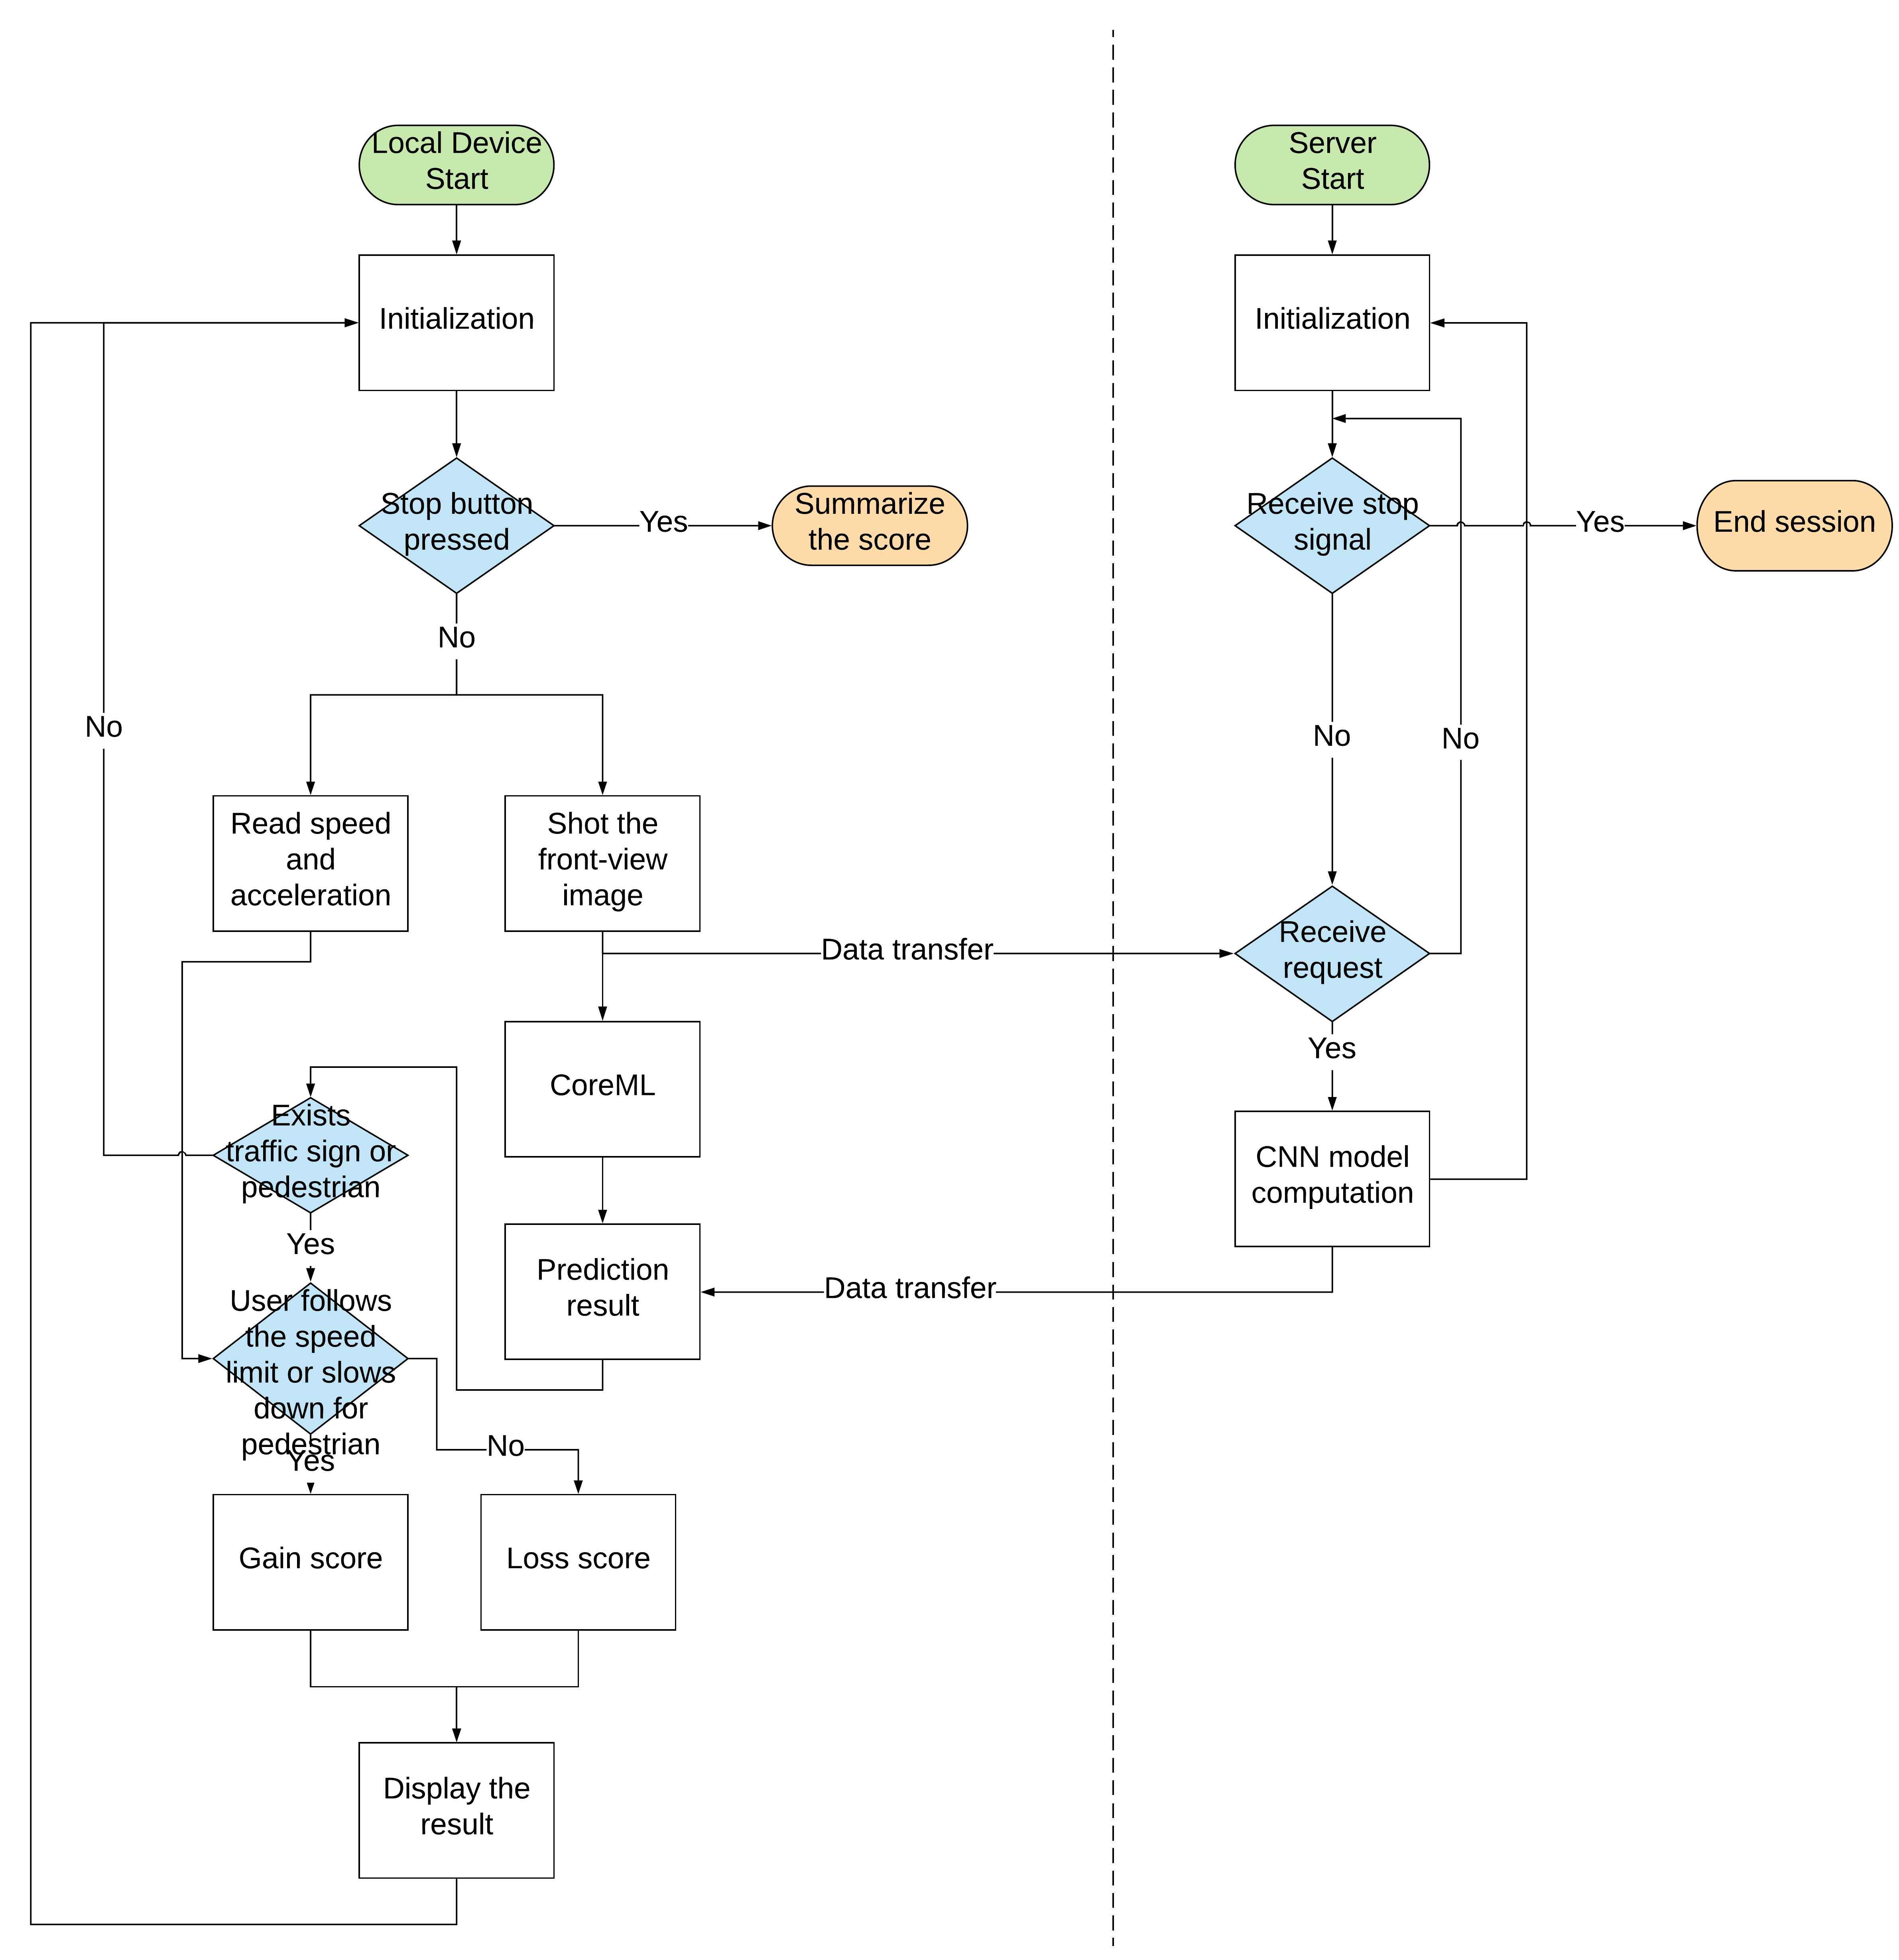
\includegraphics[width=\linewidth]{system_flowchart.png}
%   \caption{System flowchart}
% \end{figure}
\begin{figure}
  \centering
  \begin{minipage}{.4\textwidth}
    \centering
    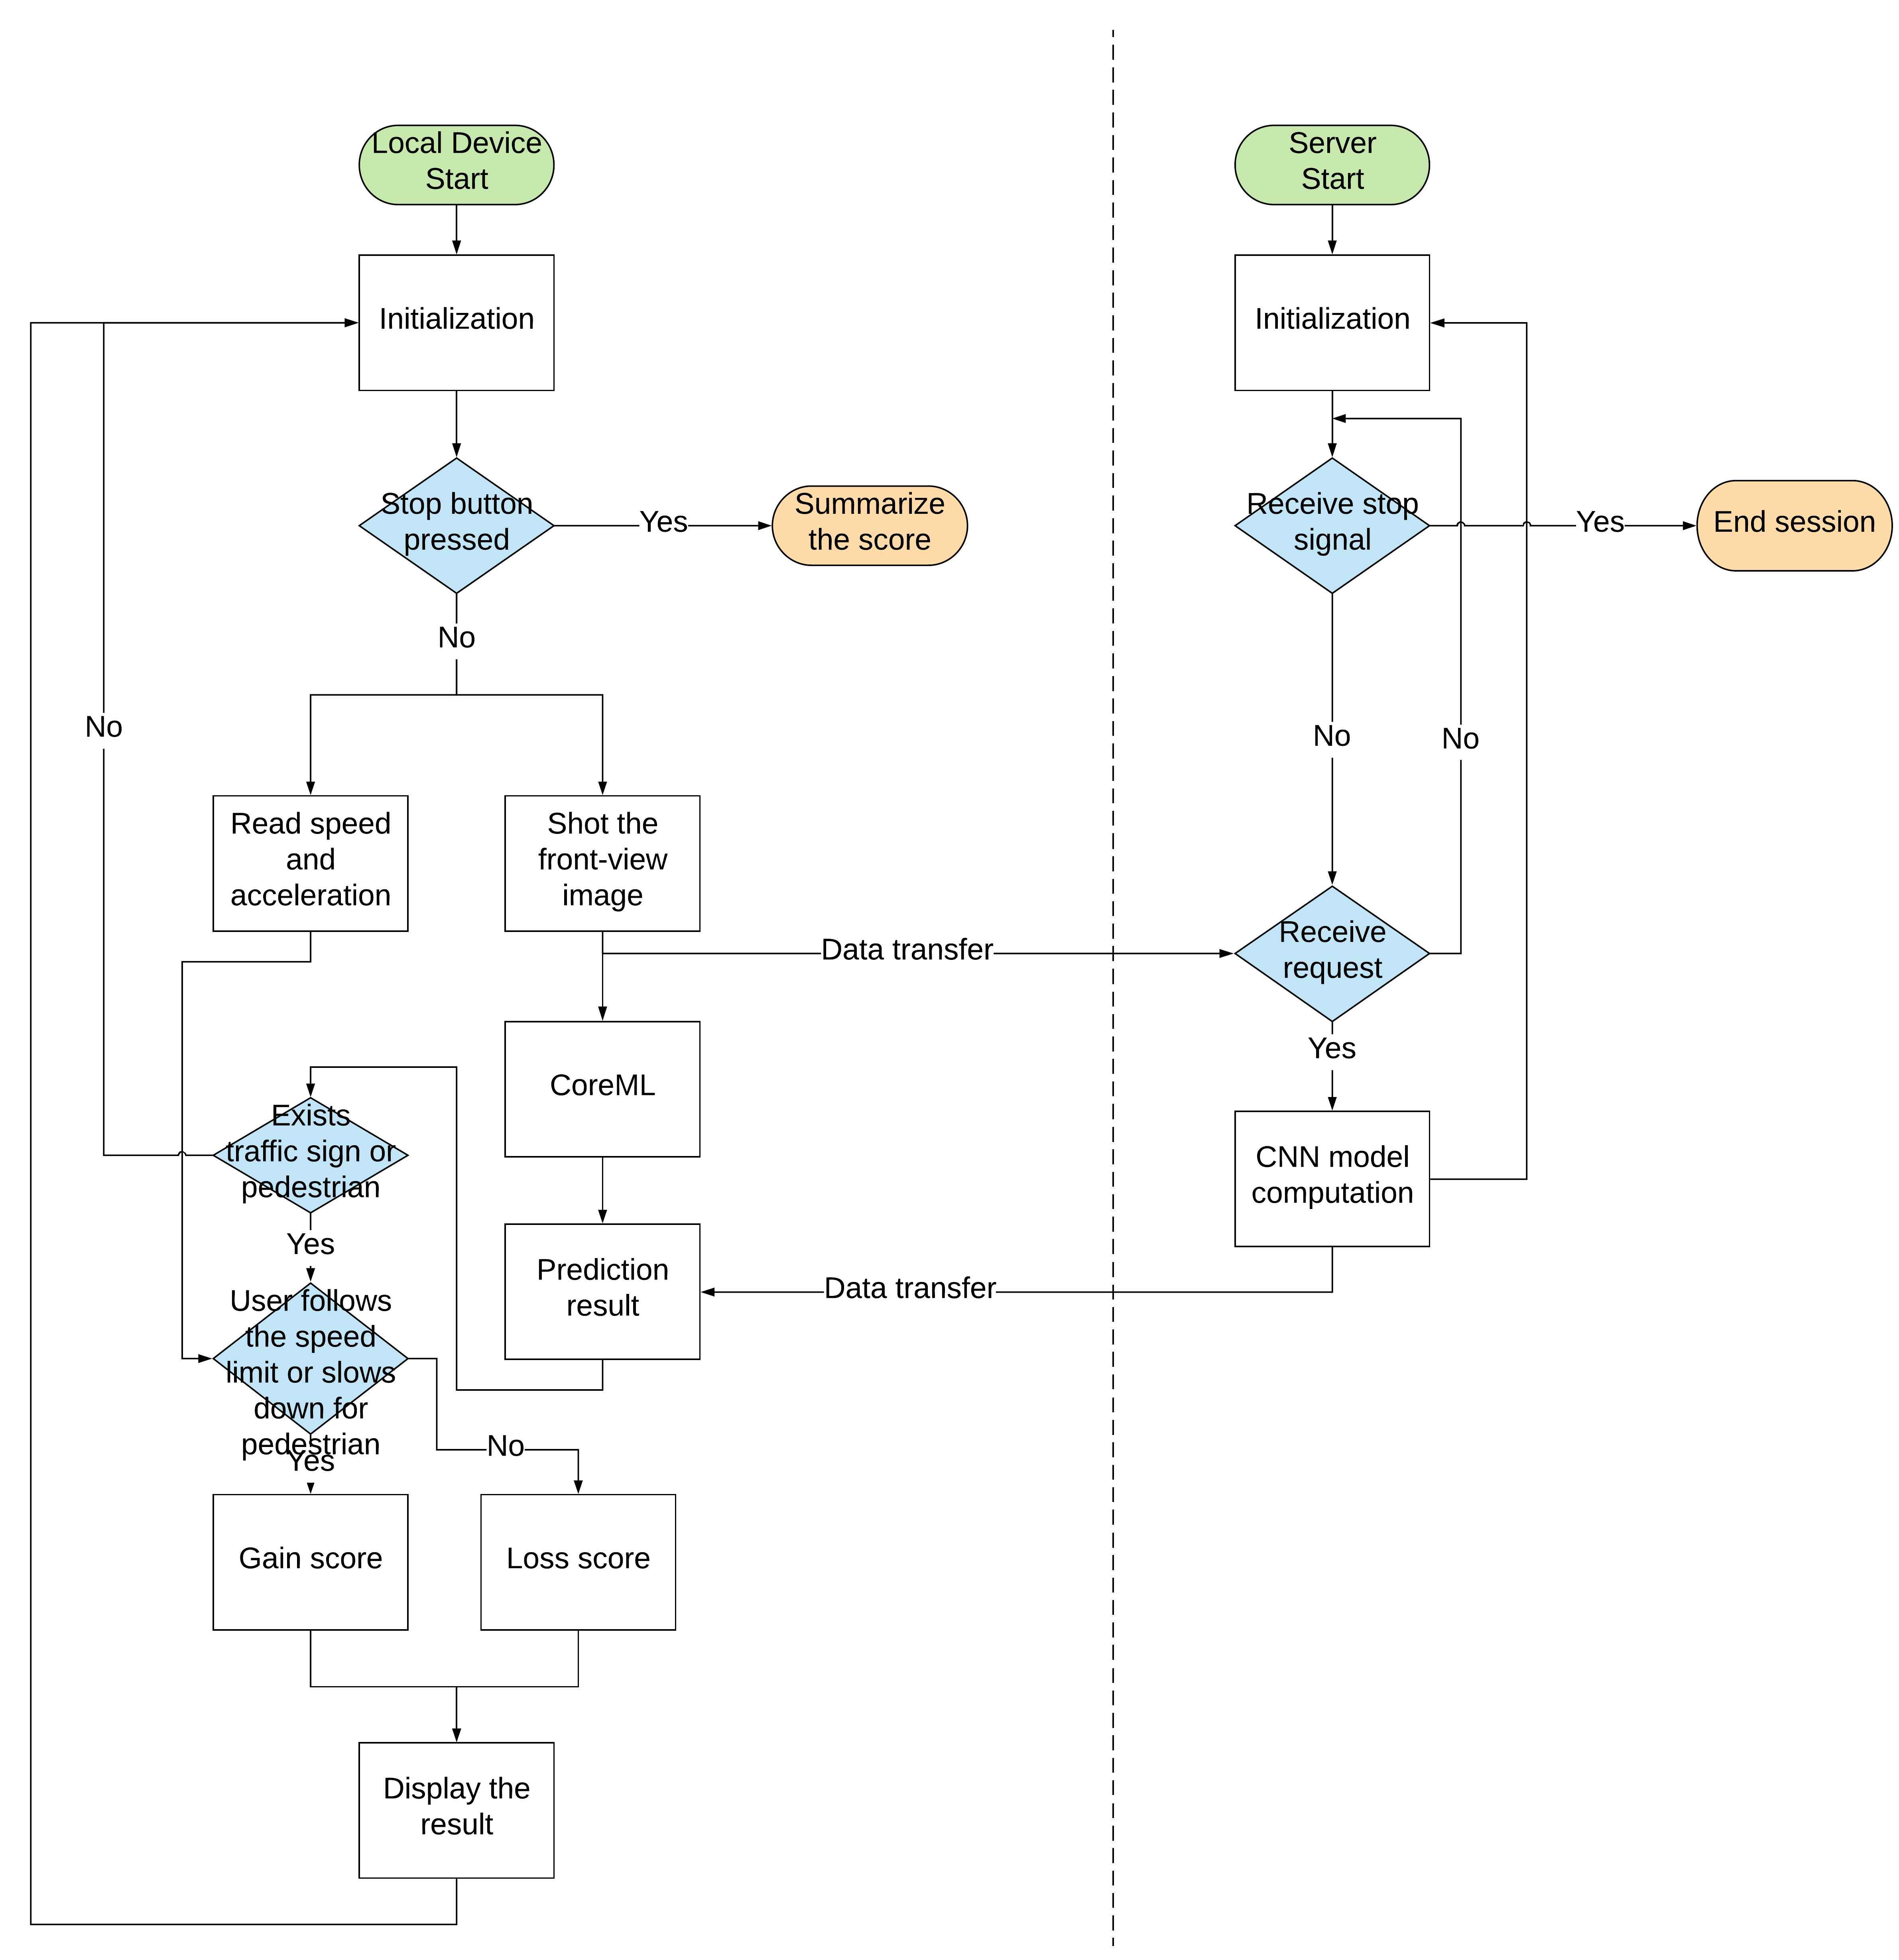
\includegraphics[width=1.2\linewidth]{system_flowchart.png}
    \caption{System design flowchart}
    \label{fig:fig_1}
  \end{minipage}
  \begin{minipage}{.4\textwidth}
    \centering
    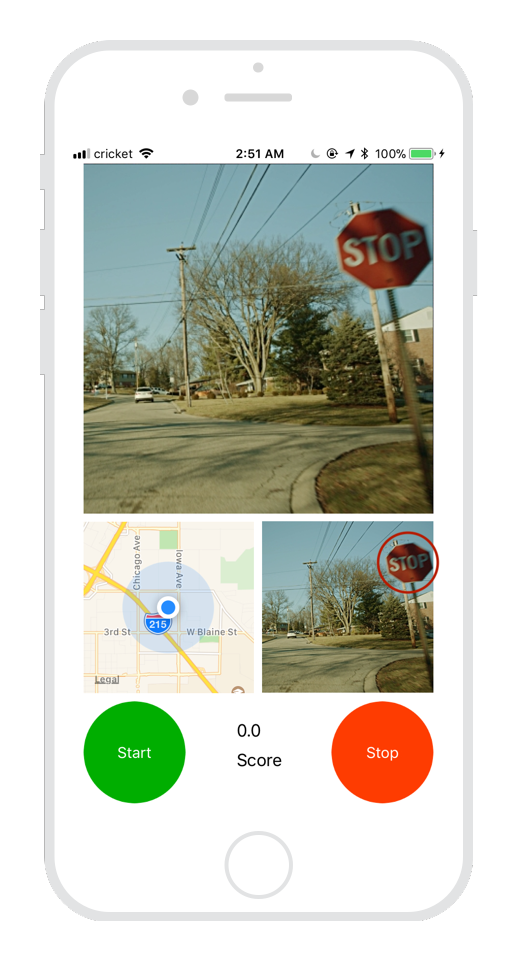
\includegraphics[width=.6\linewidth]{iOS_design.png}
    \caption{iOS app design}
    \label{fig:fig_2}
  \end{minipage}
\end{figure}
\subsection{iOS Application}
We first build a simple app for taking the front-view picture periodically, and record both the speed and acceleration at the same time via MapKit. The picture will then pass through the trained CNN model installed in the bundle, or upload to the cloud service for the prediction. The result includes whether there existed a traffic sign or traffic light in the image, and what kind of sign it is. After the translation of the speed limit is done, the app can determine if the user was over speed or not. In the end, the app would give the user a high score if he/she follows the signs and vise versa. The illustration of the app design is shown in Figure 2.

\subsection{Google Cloud Compute Engine}
We build a virtual instance with a Nvidia P100 GPU on Google Compute Engine. In the instance, we install tools like Python and CUDA and TensorFlow etc., for fast implementation of training and tuning the CNN model. The app could communicate and upload image with PHP protocol.

\subsection{Convolution Neural Network Model}
\subsubsection{Preprocessing}
Here we are using two kinds of datasets: GTSRB and LISA dataset. GTSRB contains 43 kinds of different traffic signs in Germany with 39,209 images in the set; LISA, on the other hand, contains 47 kinds of different US traffic signs with 7,855 annotations on 6,610 frames. Specifically, the images in LISA were taken in South California, which is more close to our proposed scenario.\\
The training set would first be preprocessed with normalizing, centering and histogram equalizing to help accelerating the train process in the later section. In addition, they would also be augmented, by applying rotation, mirroring and flipping, etc., to mimic more possibilities in the real world cases. And then be separated into training set, validating set and testing set. The examples of the common type of sign images in the LISA dataset is shown in Figure 3.

\begin{figure}
  \centering
  \begin{minipage}{.6\textwidth}
    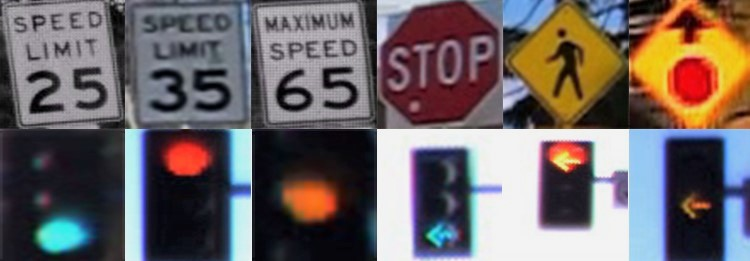
\includegraphics[width=1.0\linewidth]{dataset3.jpg}
    \caption{Images of the traffic signs}
    \label{fig:fig_3}
  \end{minipage}
\end{figure}

\subsubsection{Model Architecture}
\begin{figure}
  \centering
  \begin{minipage}{1.0\textwidth}
    \centering
    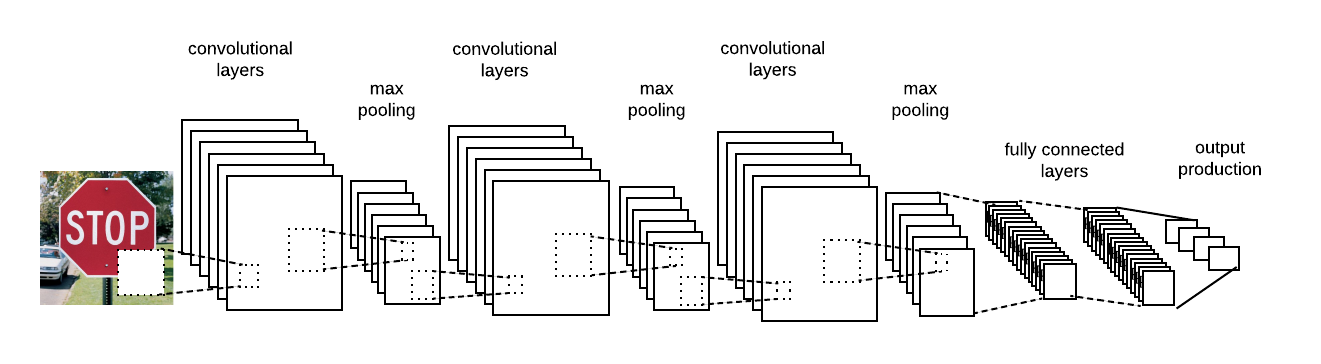
\includegraphics[width=1.0\linewidth]{conv.png}
    \caption{CNN architecture}
    \label{fig:fig_4}
  \end{minipage}
  \centering
  \begin{minipage}{0.6\textwidth}
    \centering
    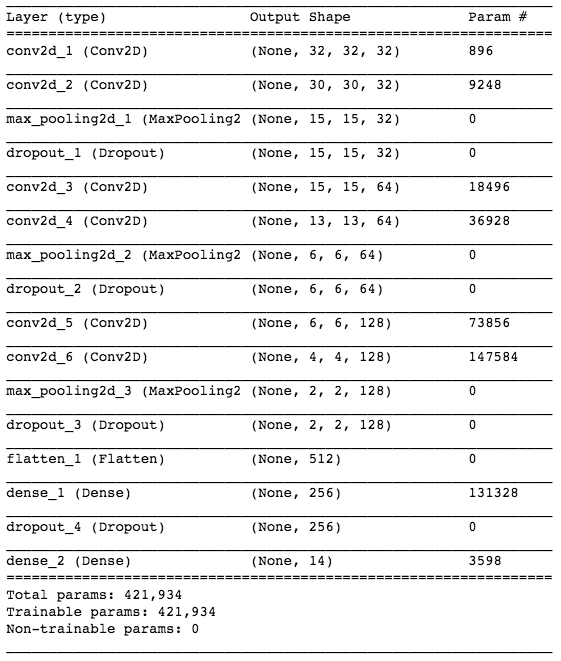
\includegraphics[width=1.0\linewidth]{archi_param.png}
    \caption{CNN architecture}
    \label{fig:fig_5}
  \end{minipage}
\end{figure}
% <old version> We would construct our own CNN model based on VGG Net [5], with a linear classifier. Specifically, we adopted VGG-5 architecture with four VGG convolution layers, a multi scale concatenate layer, two fully connected  layers and a logits layer. With the multi scale architecture that subsampling the output of each VGG block and concatenate before fully connected layer, the lower order feature in the image would still be possible to vote for the final result. While the traffic-sign feature in our scenario might serve as a small part in the whole image, this way should be a better approach to treat those and have more accurate results. Besides, we also implement Spatial Transformers for achieve invariance in scale, and the Softmax activation function for classification. 

We constructed a 6-layer CNN. The model architecture is shown in Figure 4. Each convolutional block contains 2 convolutional layers with the same number of kernel and input/output nodes. Additionally, the each block would also followed by a max-pool layer and a drop-out layer. The features extracted by the previously mentioned layers would then be feed to a fully-connected layer with dropout. Finally, the softmax layer would aggregate the result and output the probabilities of the input image with regard to each class.

\subsubsection{Model Training}
\begin{figure}
  \centering
  \begin{minipage}{.42\textwidth}
    \centering
    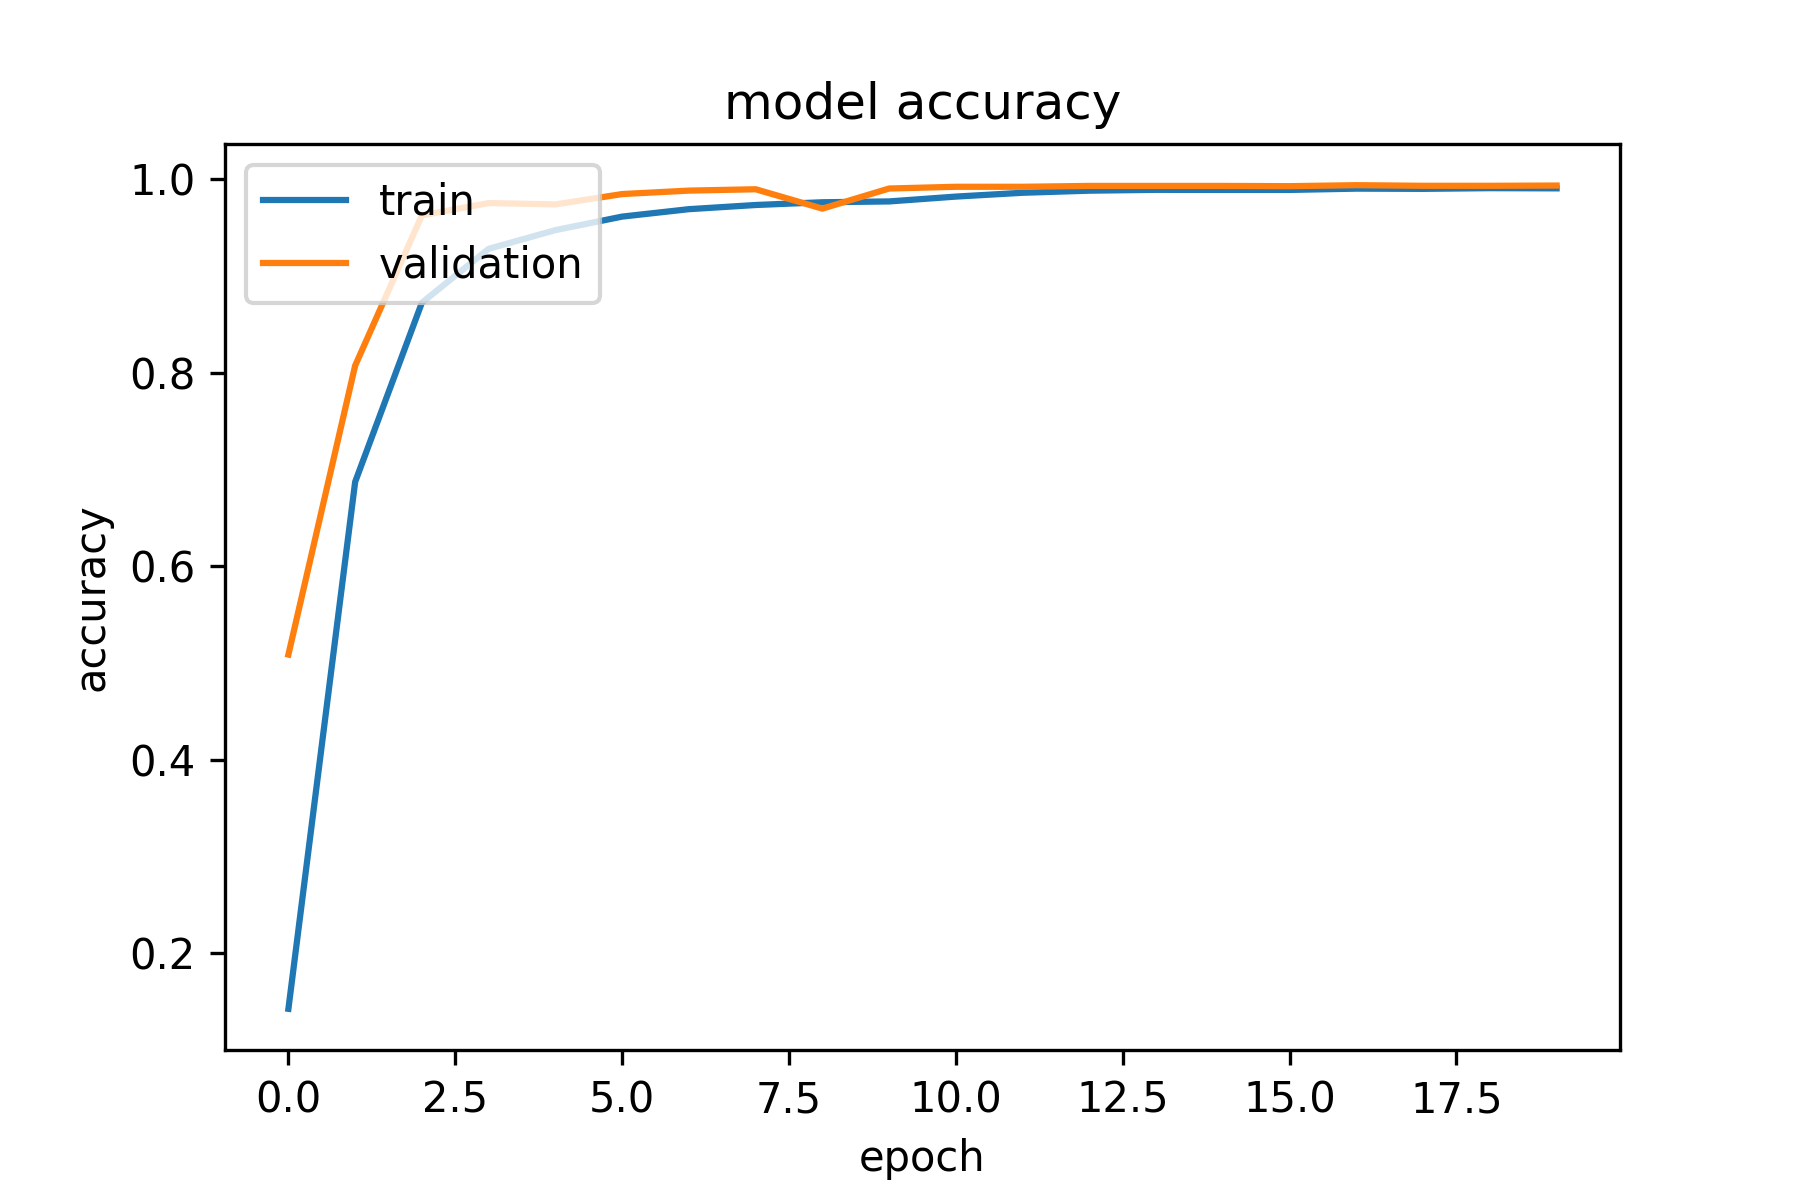
\includegraphics[width=0.95\linewidth]{acc_f.png}
    \caption{Training accuracy with GTSRB}
    \label{fig:fig_6}
  \end{minipage}
  \begin{minipage}{.42\textwidth}
    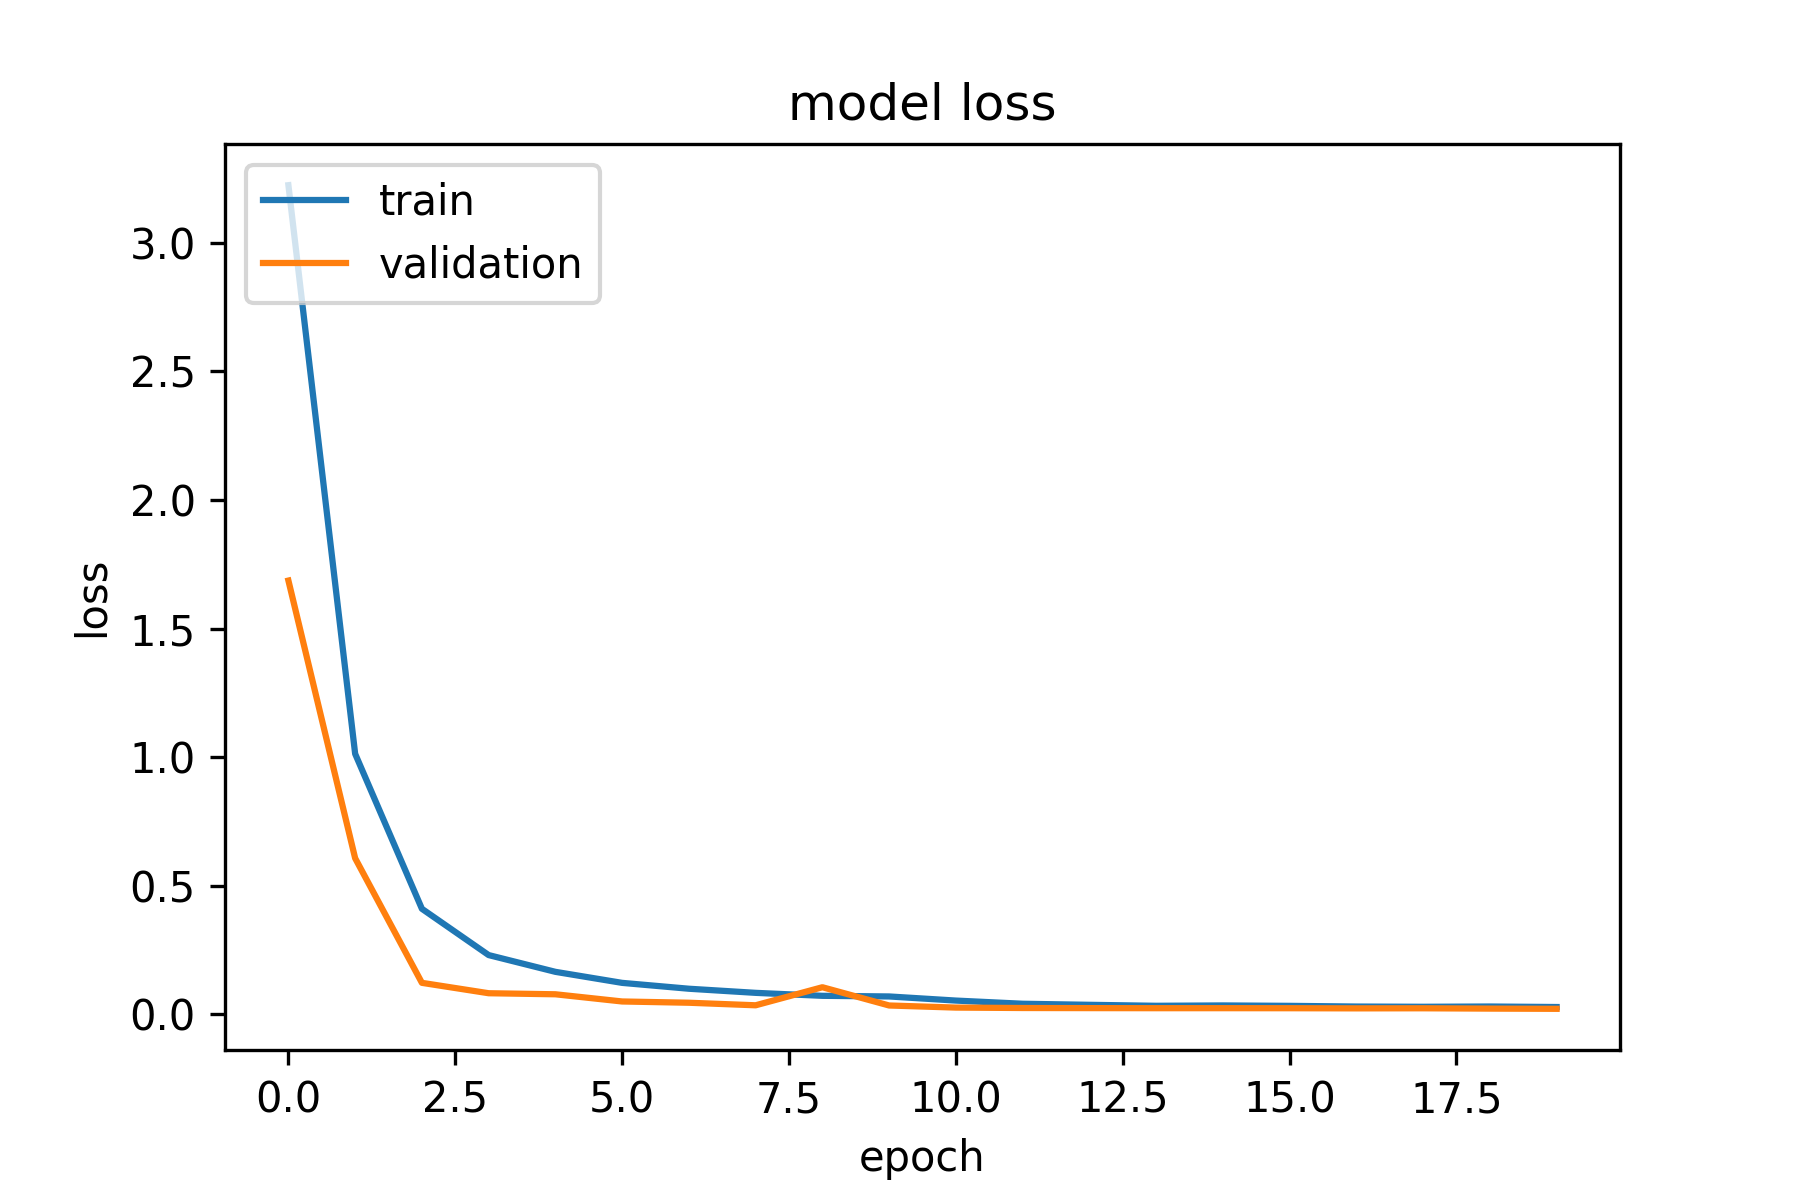
\includegraphics[width=0.95\linewidth]{loss_f.png}
    \centering
    \caption{Training accuracy with GTSRB}
    \label{fig:fig_7}
  \end{minipage}
  \centering
  \begin{minipage}{.42\textwidth}
  	\centering
    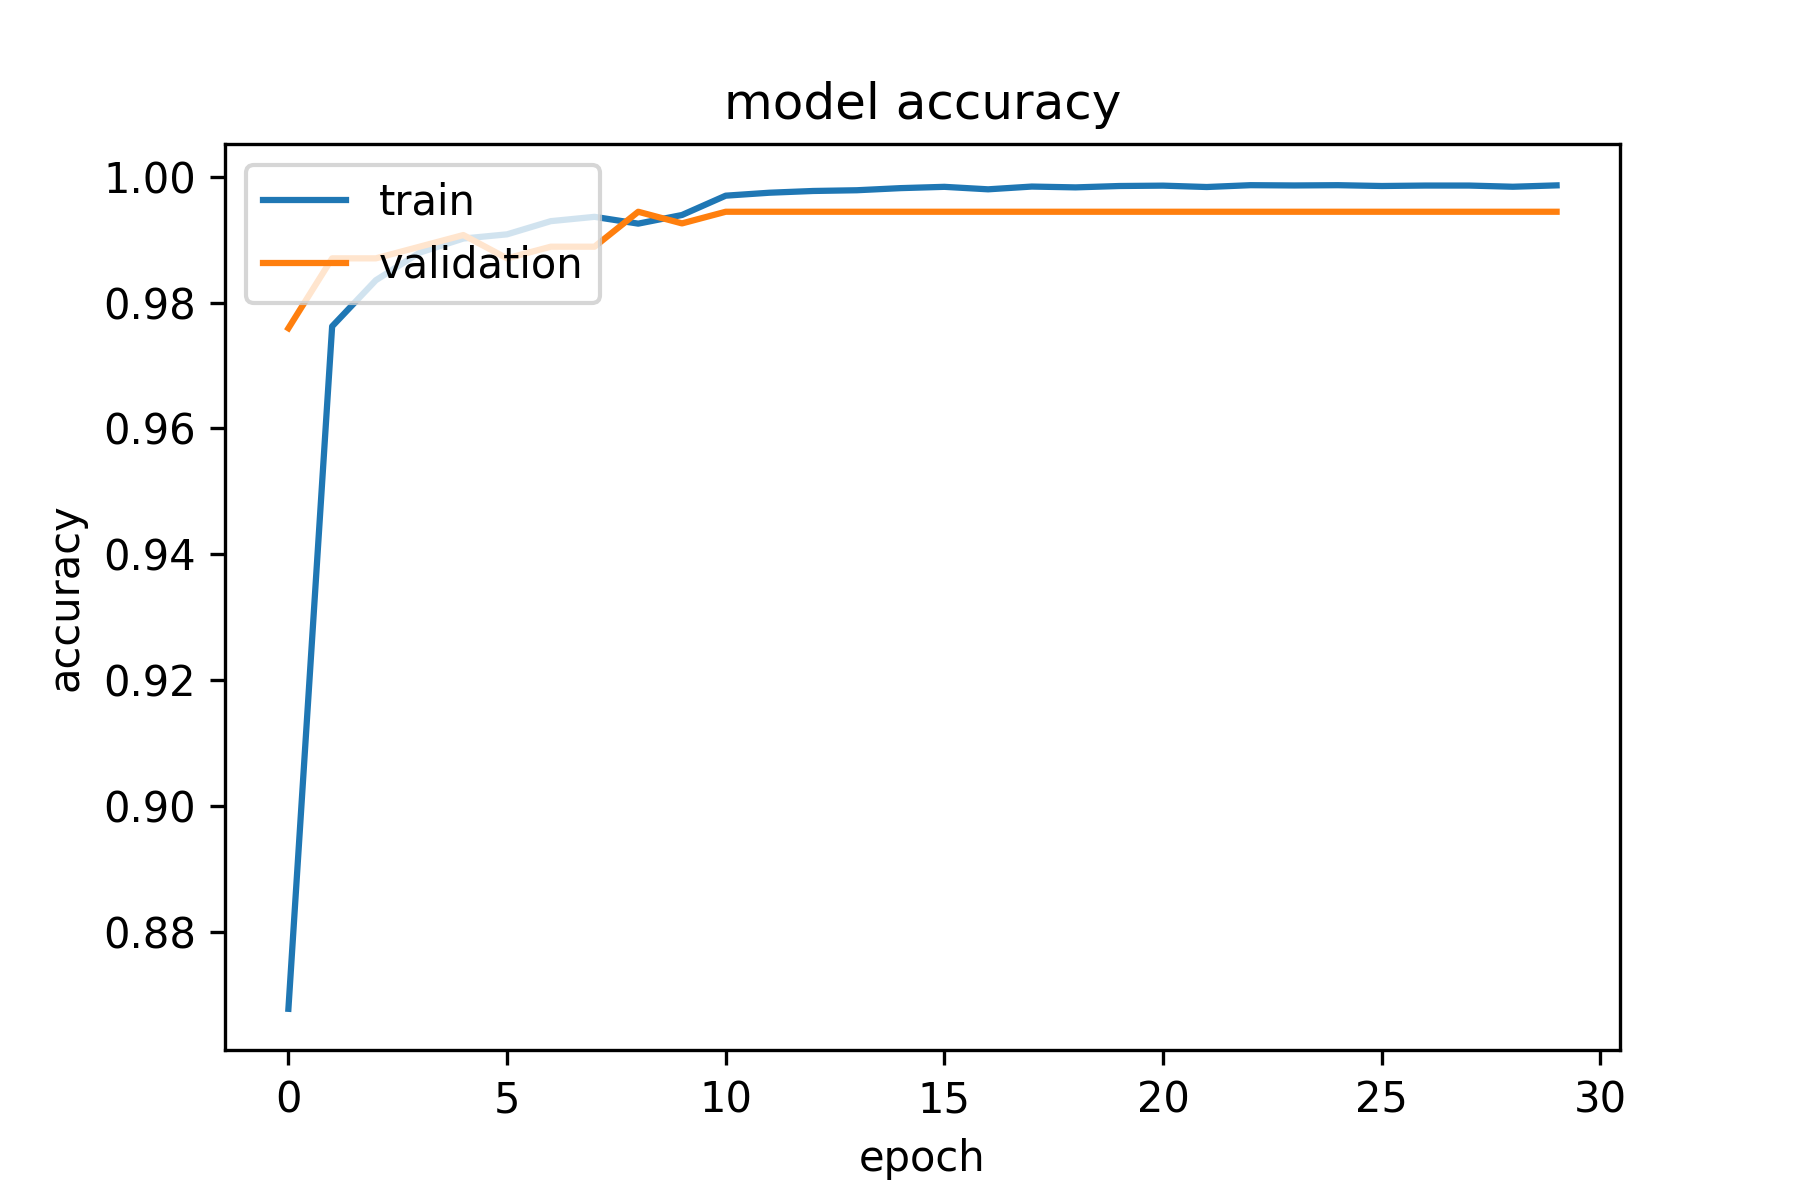
\includegraphics[width=0.95\linewidth]{model_accuracy.png}
    \caption{Training accuracy with LISA traffic sign dataset}
    \label{fig:fig_8}
  \end{minipage}
  \begin{minipage}{.42\textwidth}
    \centering
    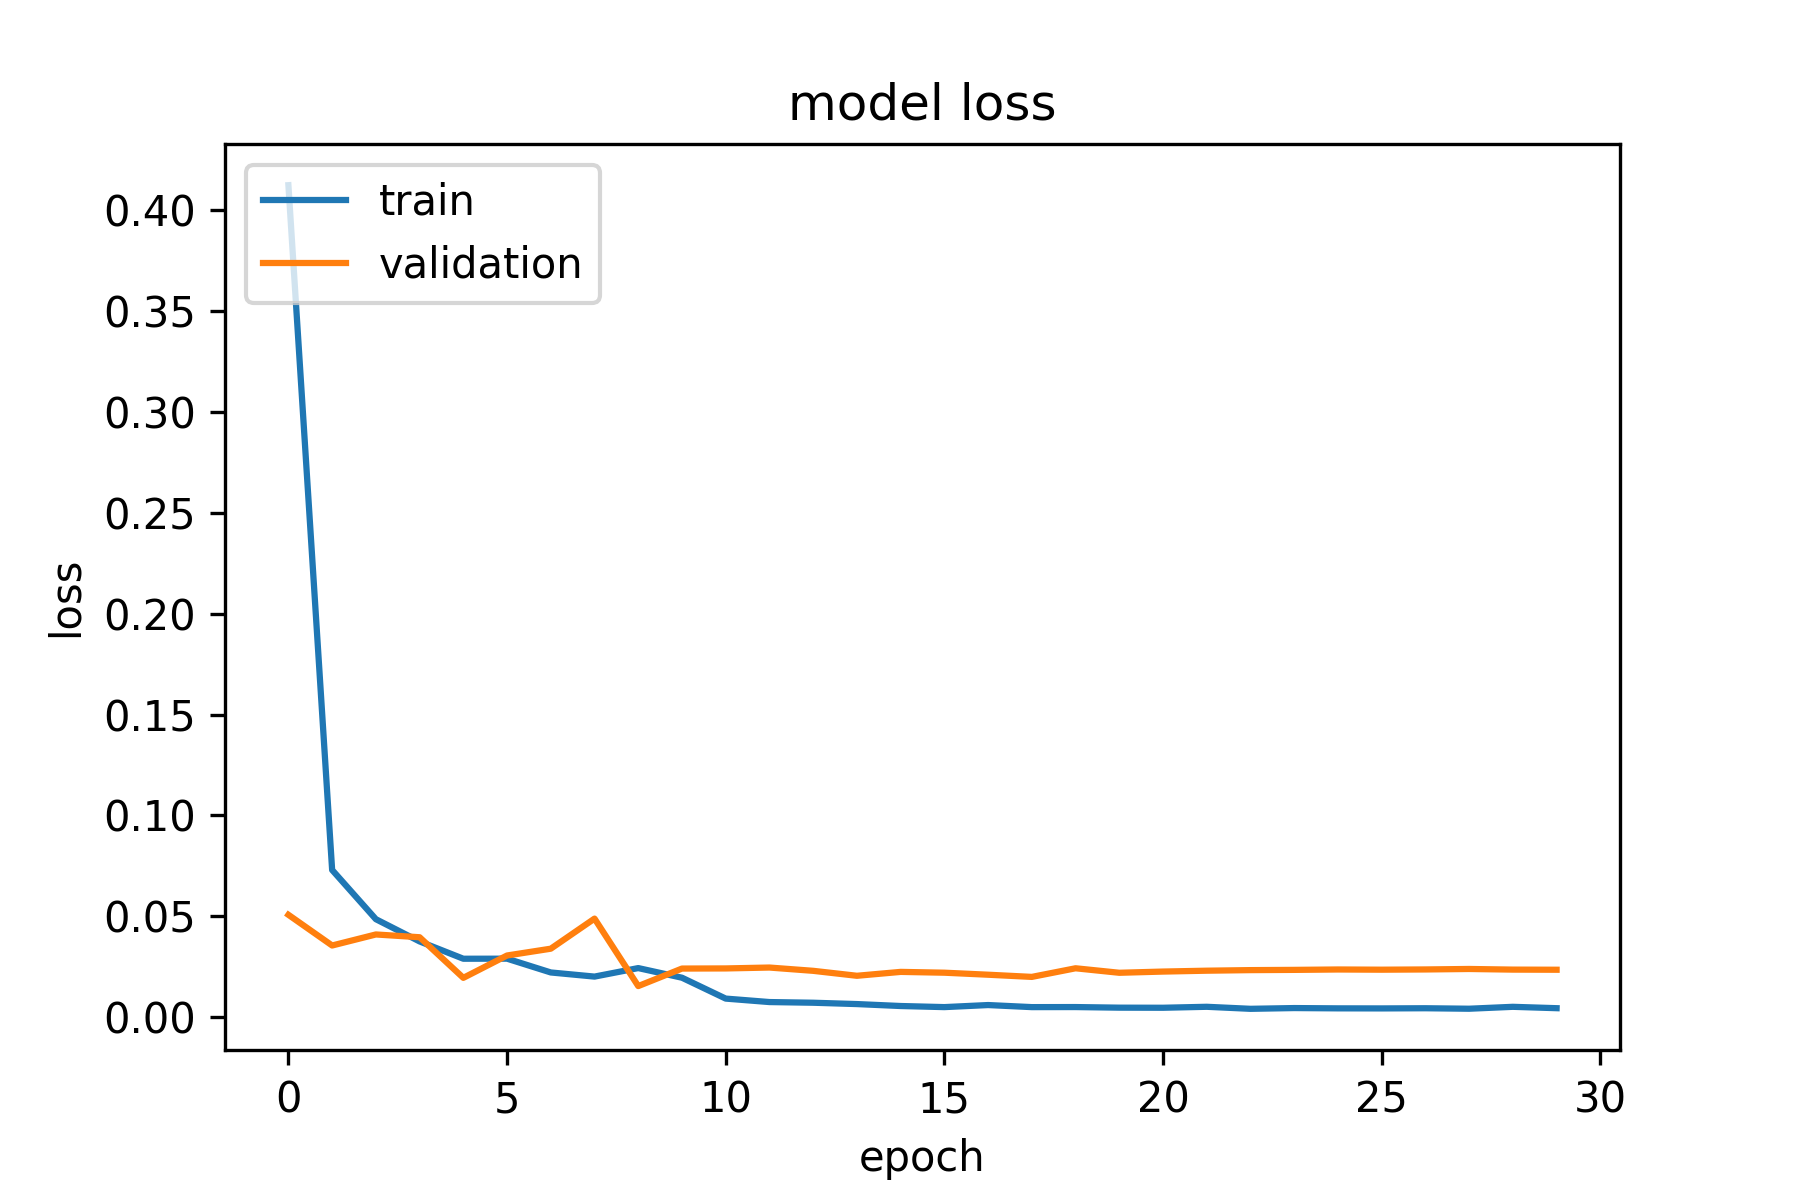
\includegraphics[width=0.95\linewidth]{model_loss.png}
    \caption{Training accuracy with LISA traffic sign dataset}
    \label{fig:fig_9}
  \end{minipage}
  \centering
  \begin{minipage}{.42\textwidth}
  	\centering
    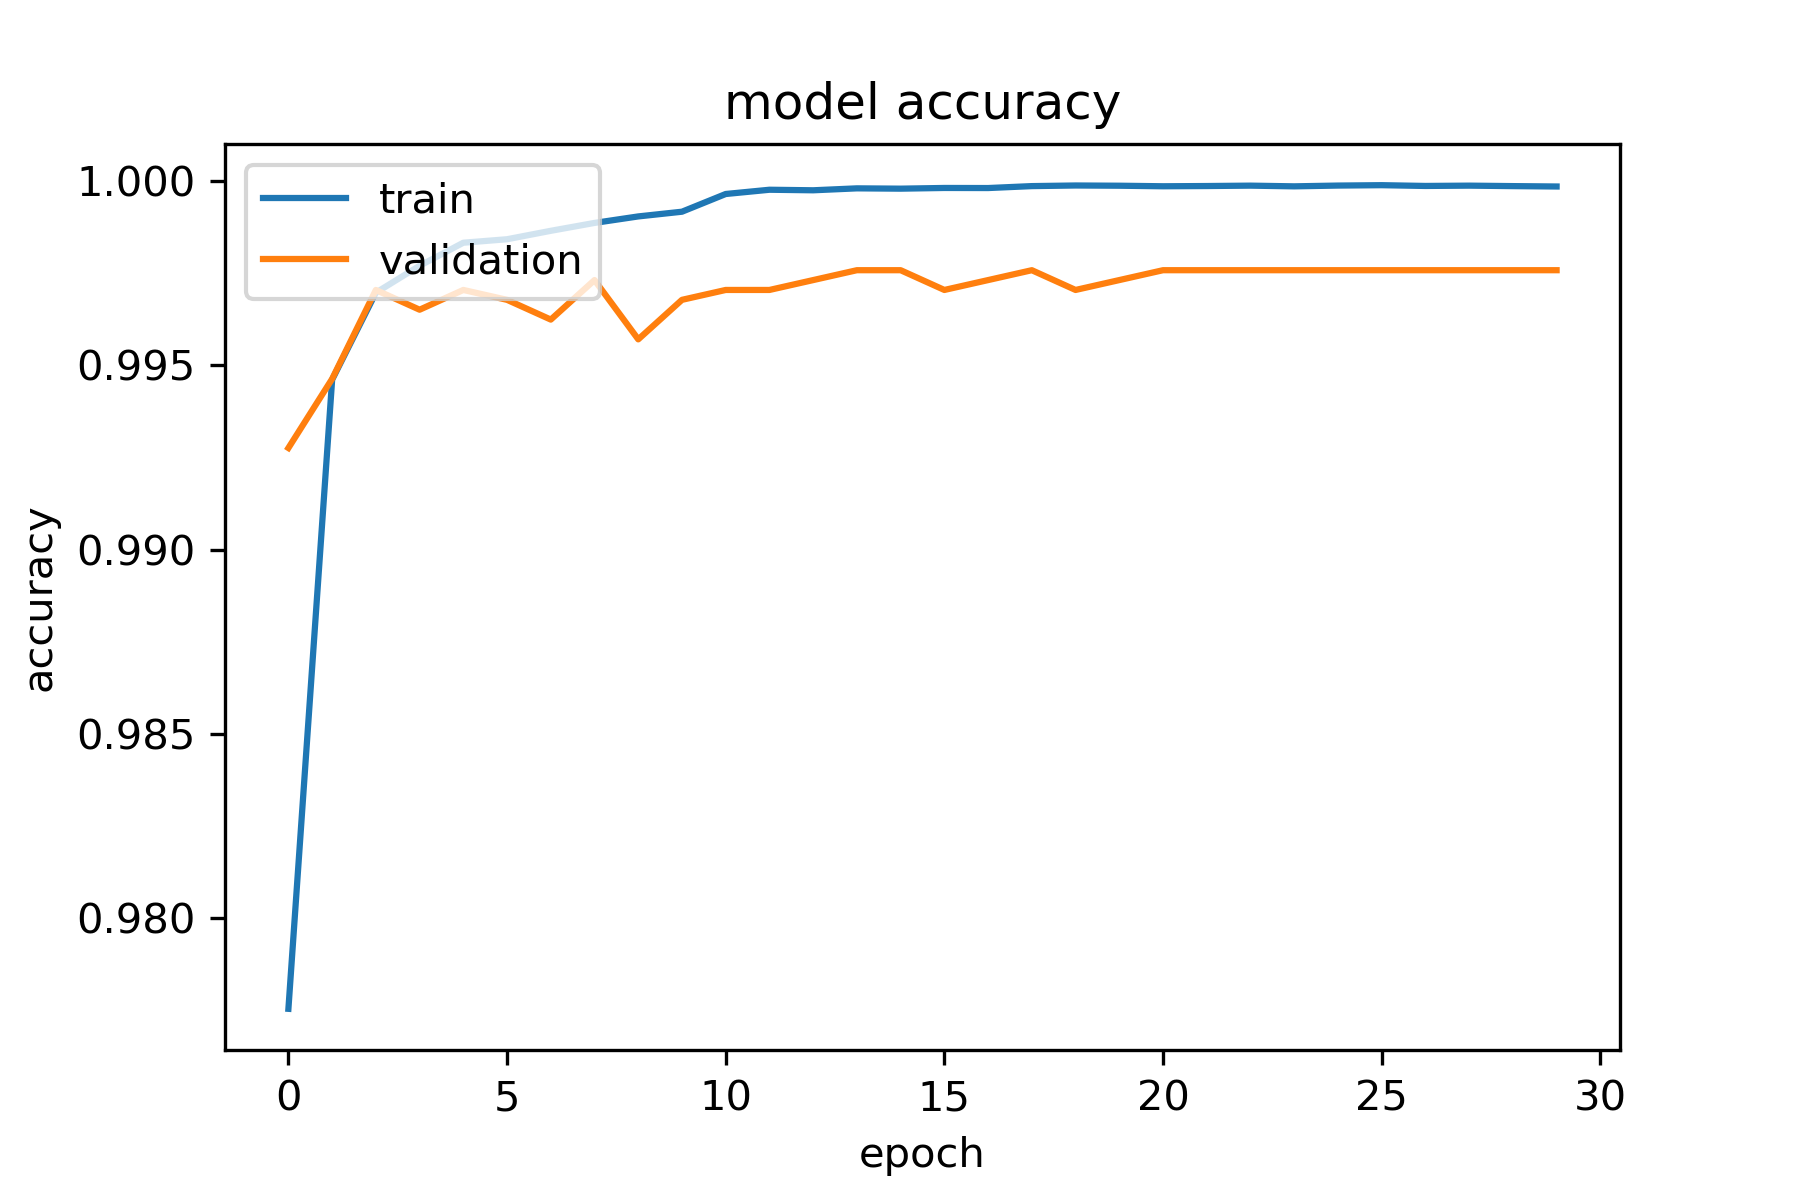
\includegraphics[width=0.95\linewidth]{model_accuracy_traffic_light.png}
    \caption{Training accuracy with LISA traffic light dataset}
    \label{fig:fig_10}
  \end{minipage}
  \begin{minipage}{.42\textwidth}
    \centering
    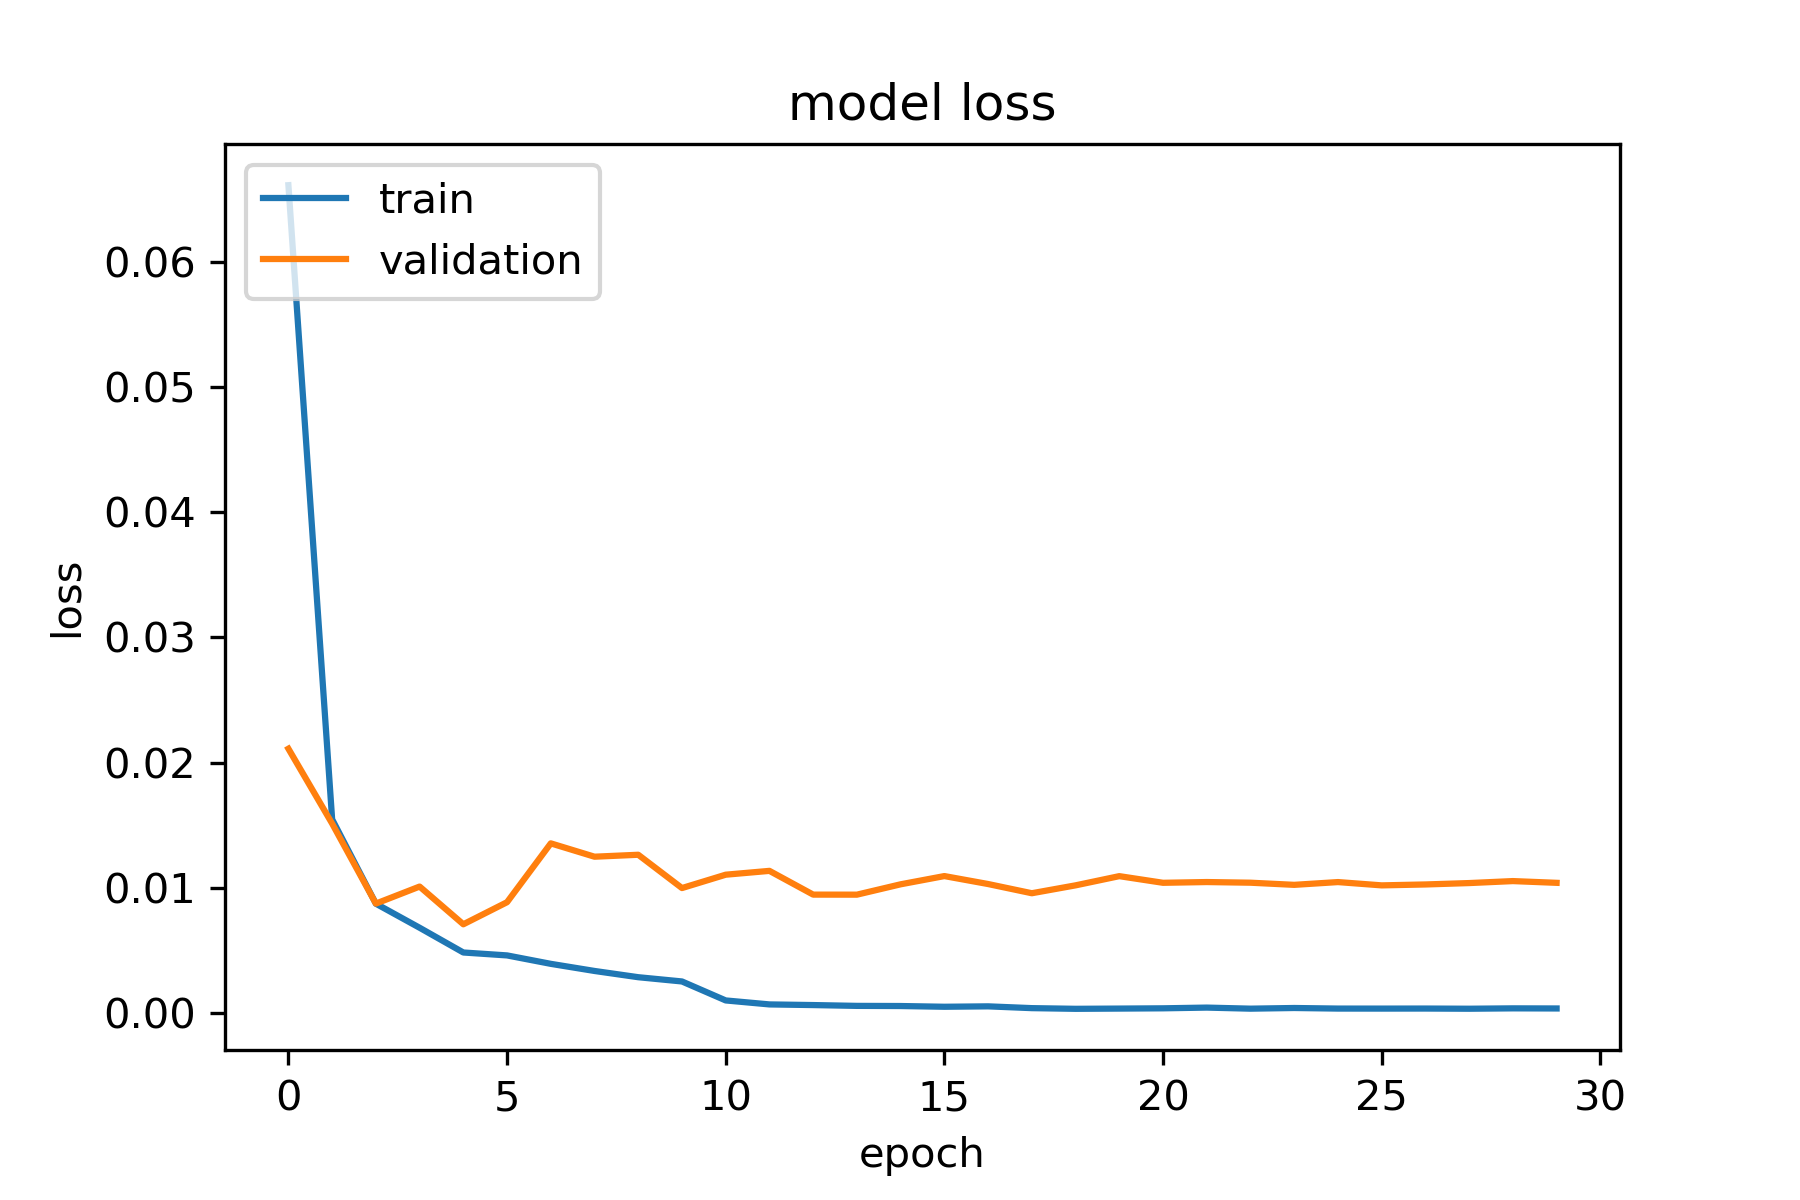
\includegraphics[width=0.95\linewidth]{model_loss_traffic_light.png}
    \caption{Training accuracy with LISA traffic light dataset}
    \label{fig:fig_11}
  \end{minipage}
\end{figure}
The models was trained by training dataset with augmented images, tuned with Stochastic Gradient Descent (SGD) and momentum to speed-up the training process. The training process took 2052 seconds per epoch with GTSRB dataset, 30 seconds per epoch with LISA traffic sign dataset, 201 seconds per epoch with LISA traffic light dataset. The training accuracy and loss by each epoch with three kinds of dataset was shown in Figure 5 to Figure 10. Among them, we can see the training accuracy could even reach 100\%, and validation accuracy could be higher than 95\%. 
% \section{Proceeding works}
% After completing the training process, we would conduct the model into experiment. Our model would be translate into coreML model for implementation on the iOS device. To test computation speed and accuracy both on the cloud service and local device. On the other hand, we would also work on speed-up and optimize the model for securing real-time scenario.
% \subsubsection{Model Testing}
\section{Evaluation}
\begin{table}
  \caption{CNN model test result}
  \label{table_1}
  \begin{center}
    \begin{tabular}{ | l | c | c |}
      \hline
      Dataset & No. of classes & Test accuracy \\ \hline
      GTSRB & 43 & 96.4\% \\ \hline
      LISA Traffic Sign & 14 & 99.8\% \\ \hline
      LISA Traffic Light & 6 & 99.5\% \\
      \hline
    \end{tabular}
  \end{center}
\end{table}

\begin{figure}
  \centering
  \begin{minipage}{.5\textwidth}
    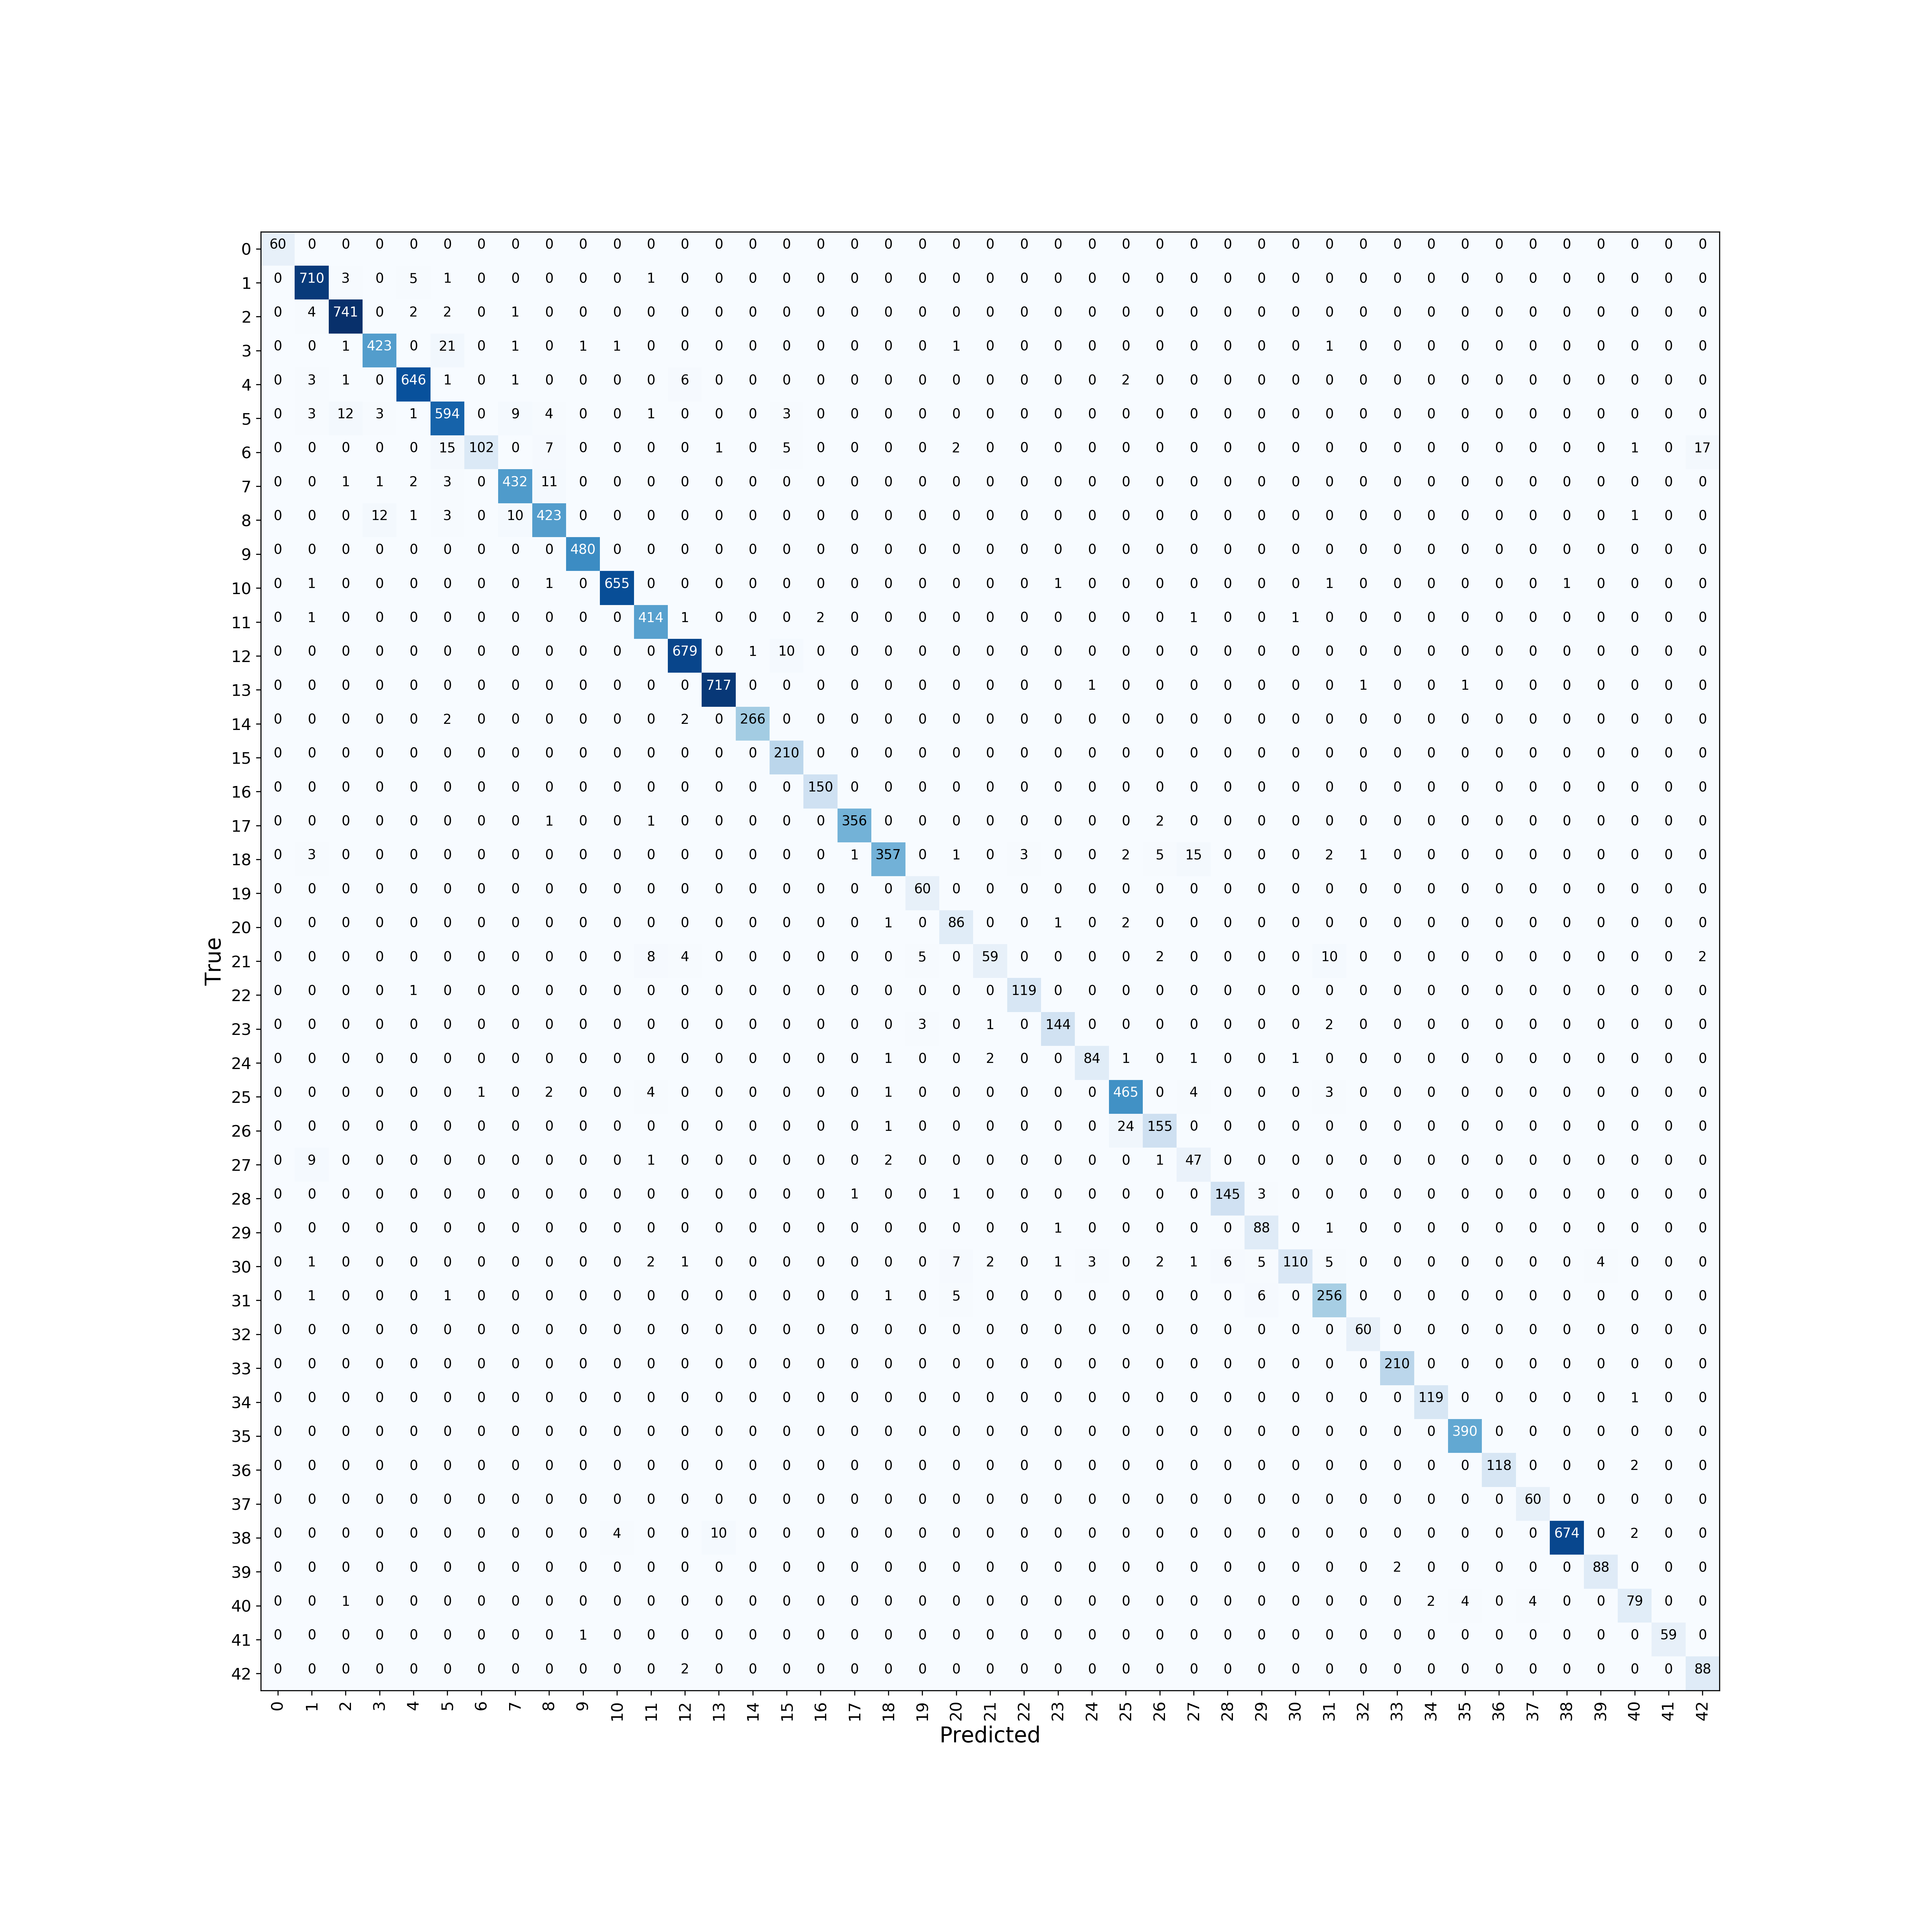
\includegraphics[width=1.0\linewidth]{confusion_matrix_f.png}
    \centering
    \caption{Testing confusion matrix with GTSRB}
    \label{fig:fig_11}
  \end{minipage}
  \begin{minipage}{.5\textwidth}
    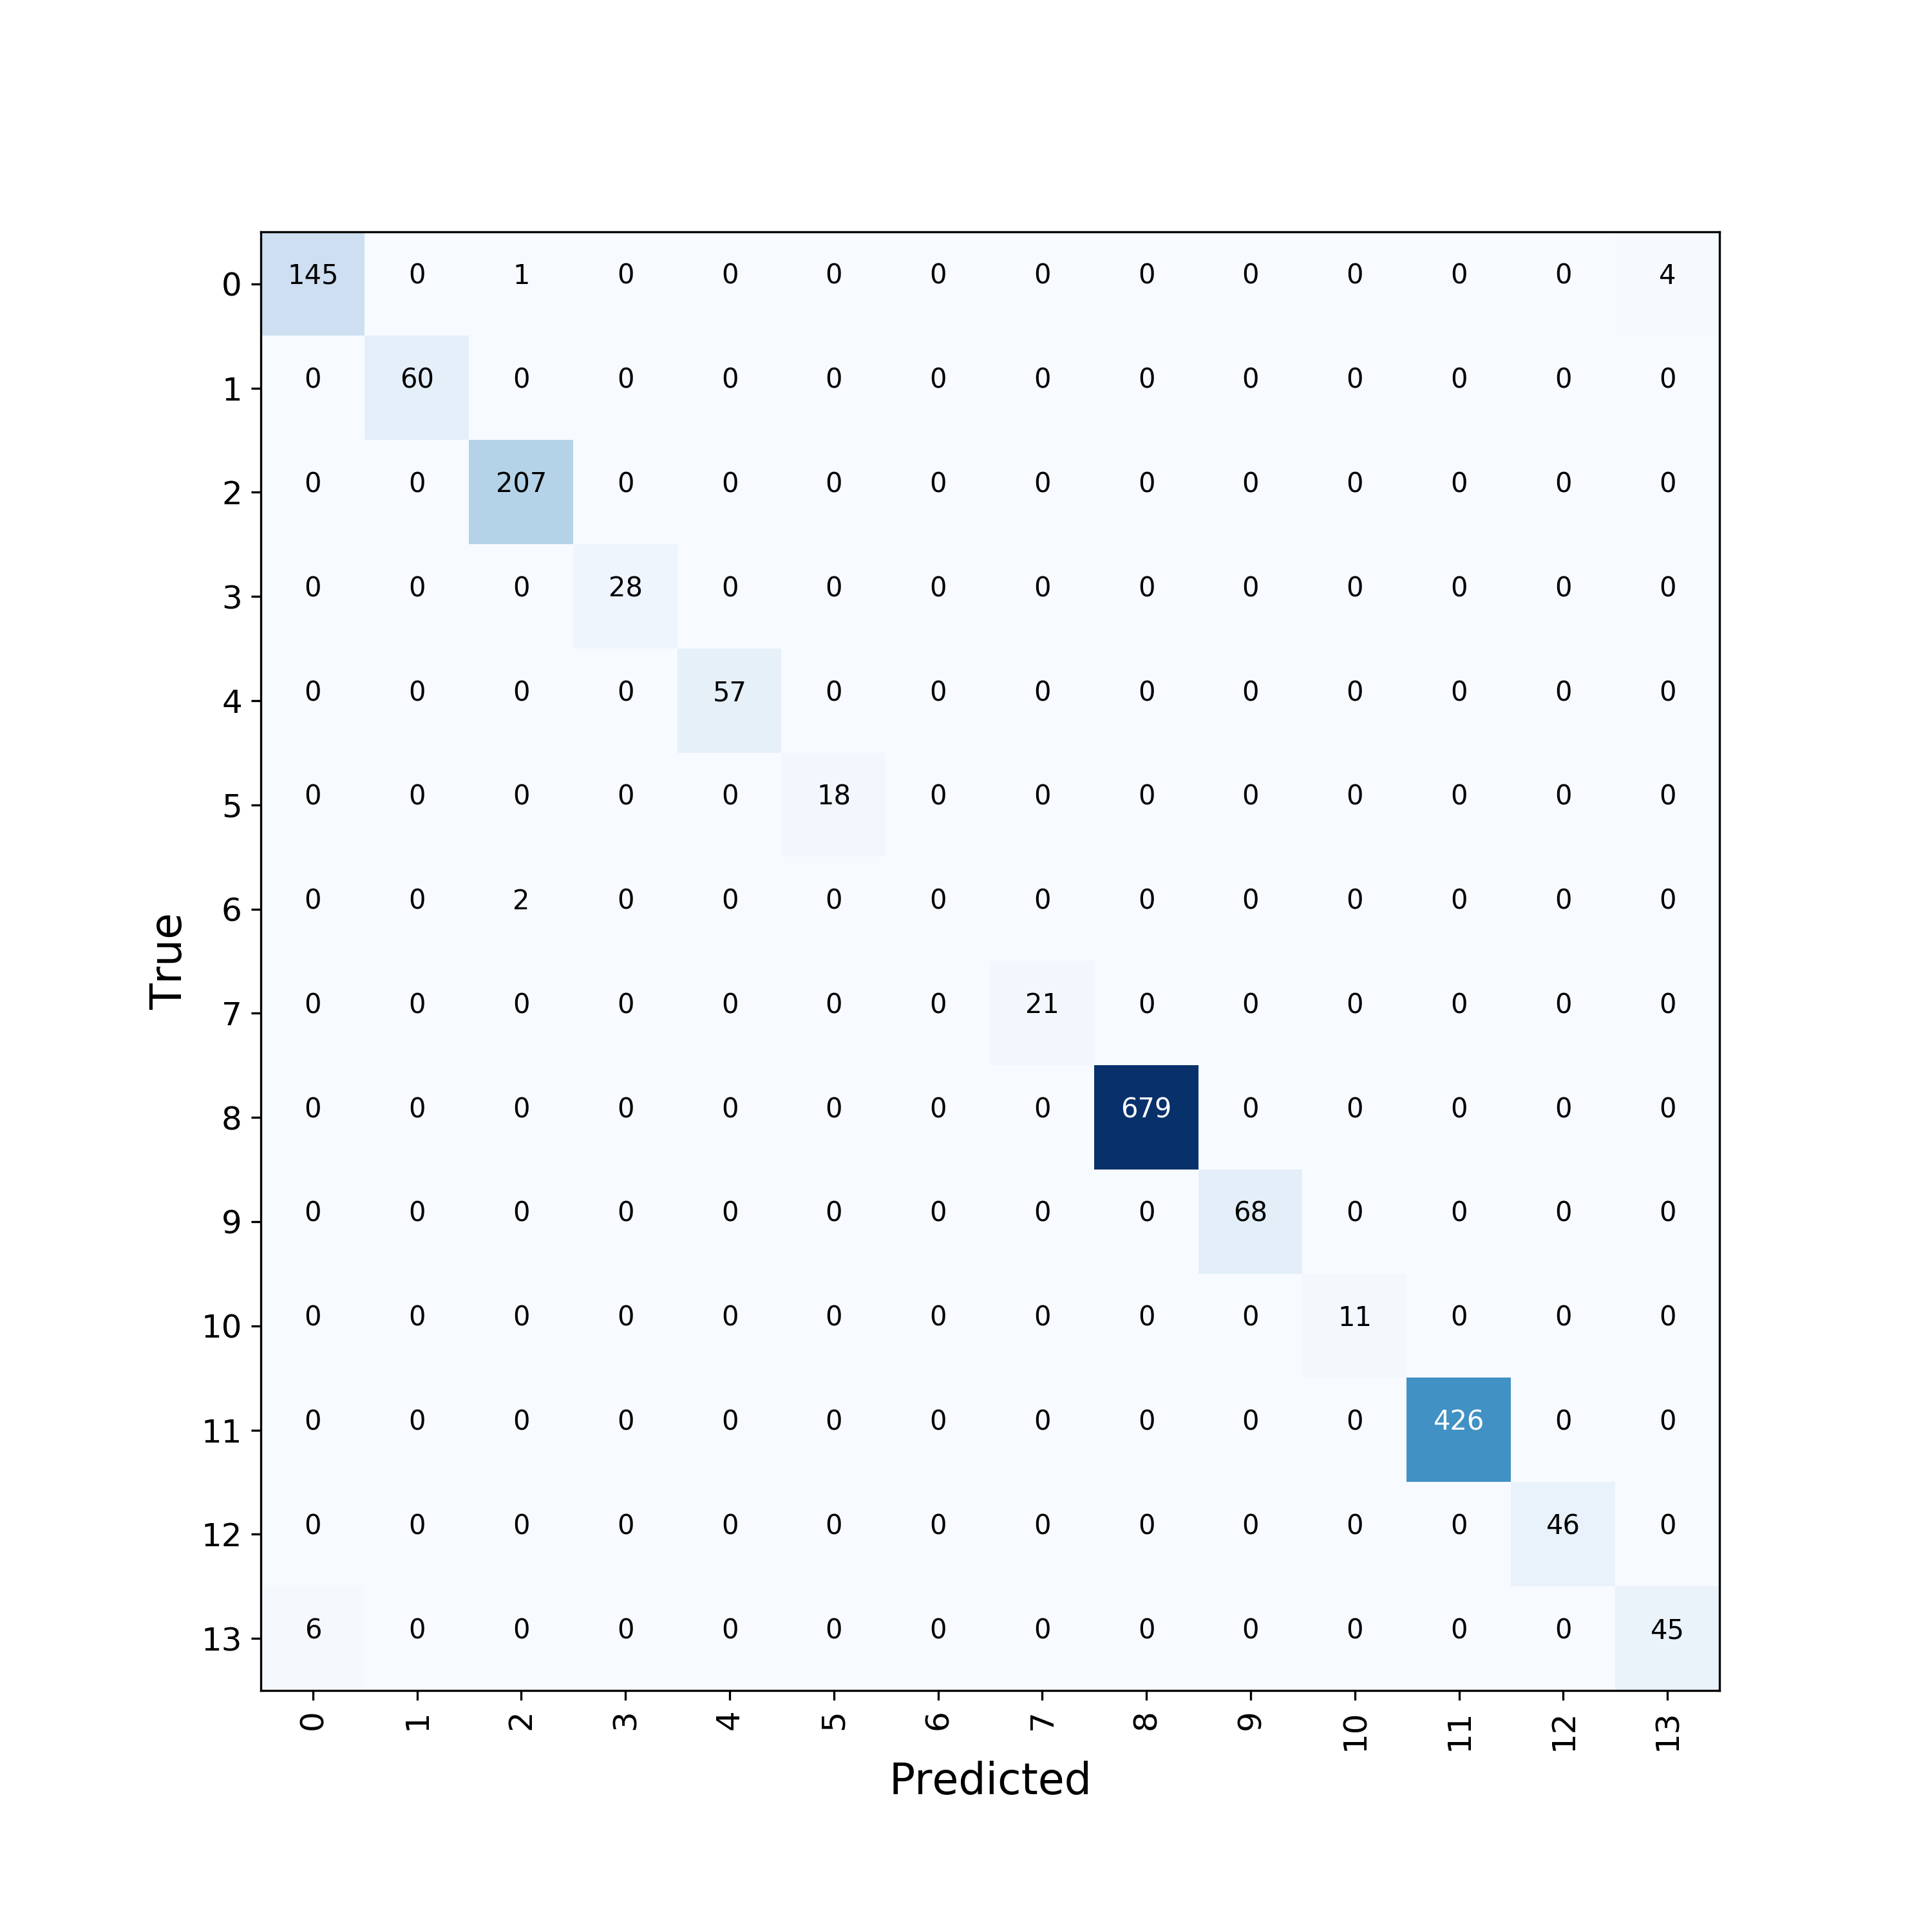
\includegraphics[width=1.0\linewidth]{confusion_matrix.png}
    \centering
    \caption{Testing confusion matrix with LISA traffic sign}
    \label{fig:fig_12}
  \end{minipage}
  \begin{minipage}{.5\textwidth}
    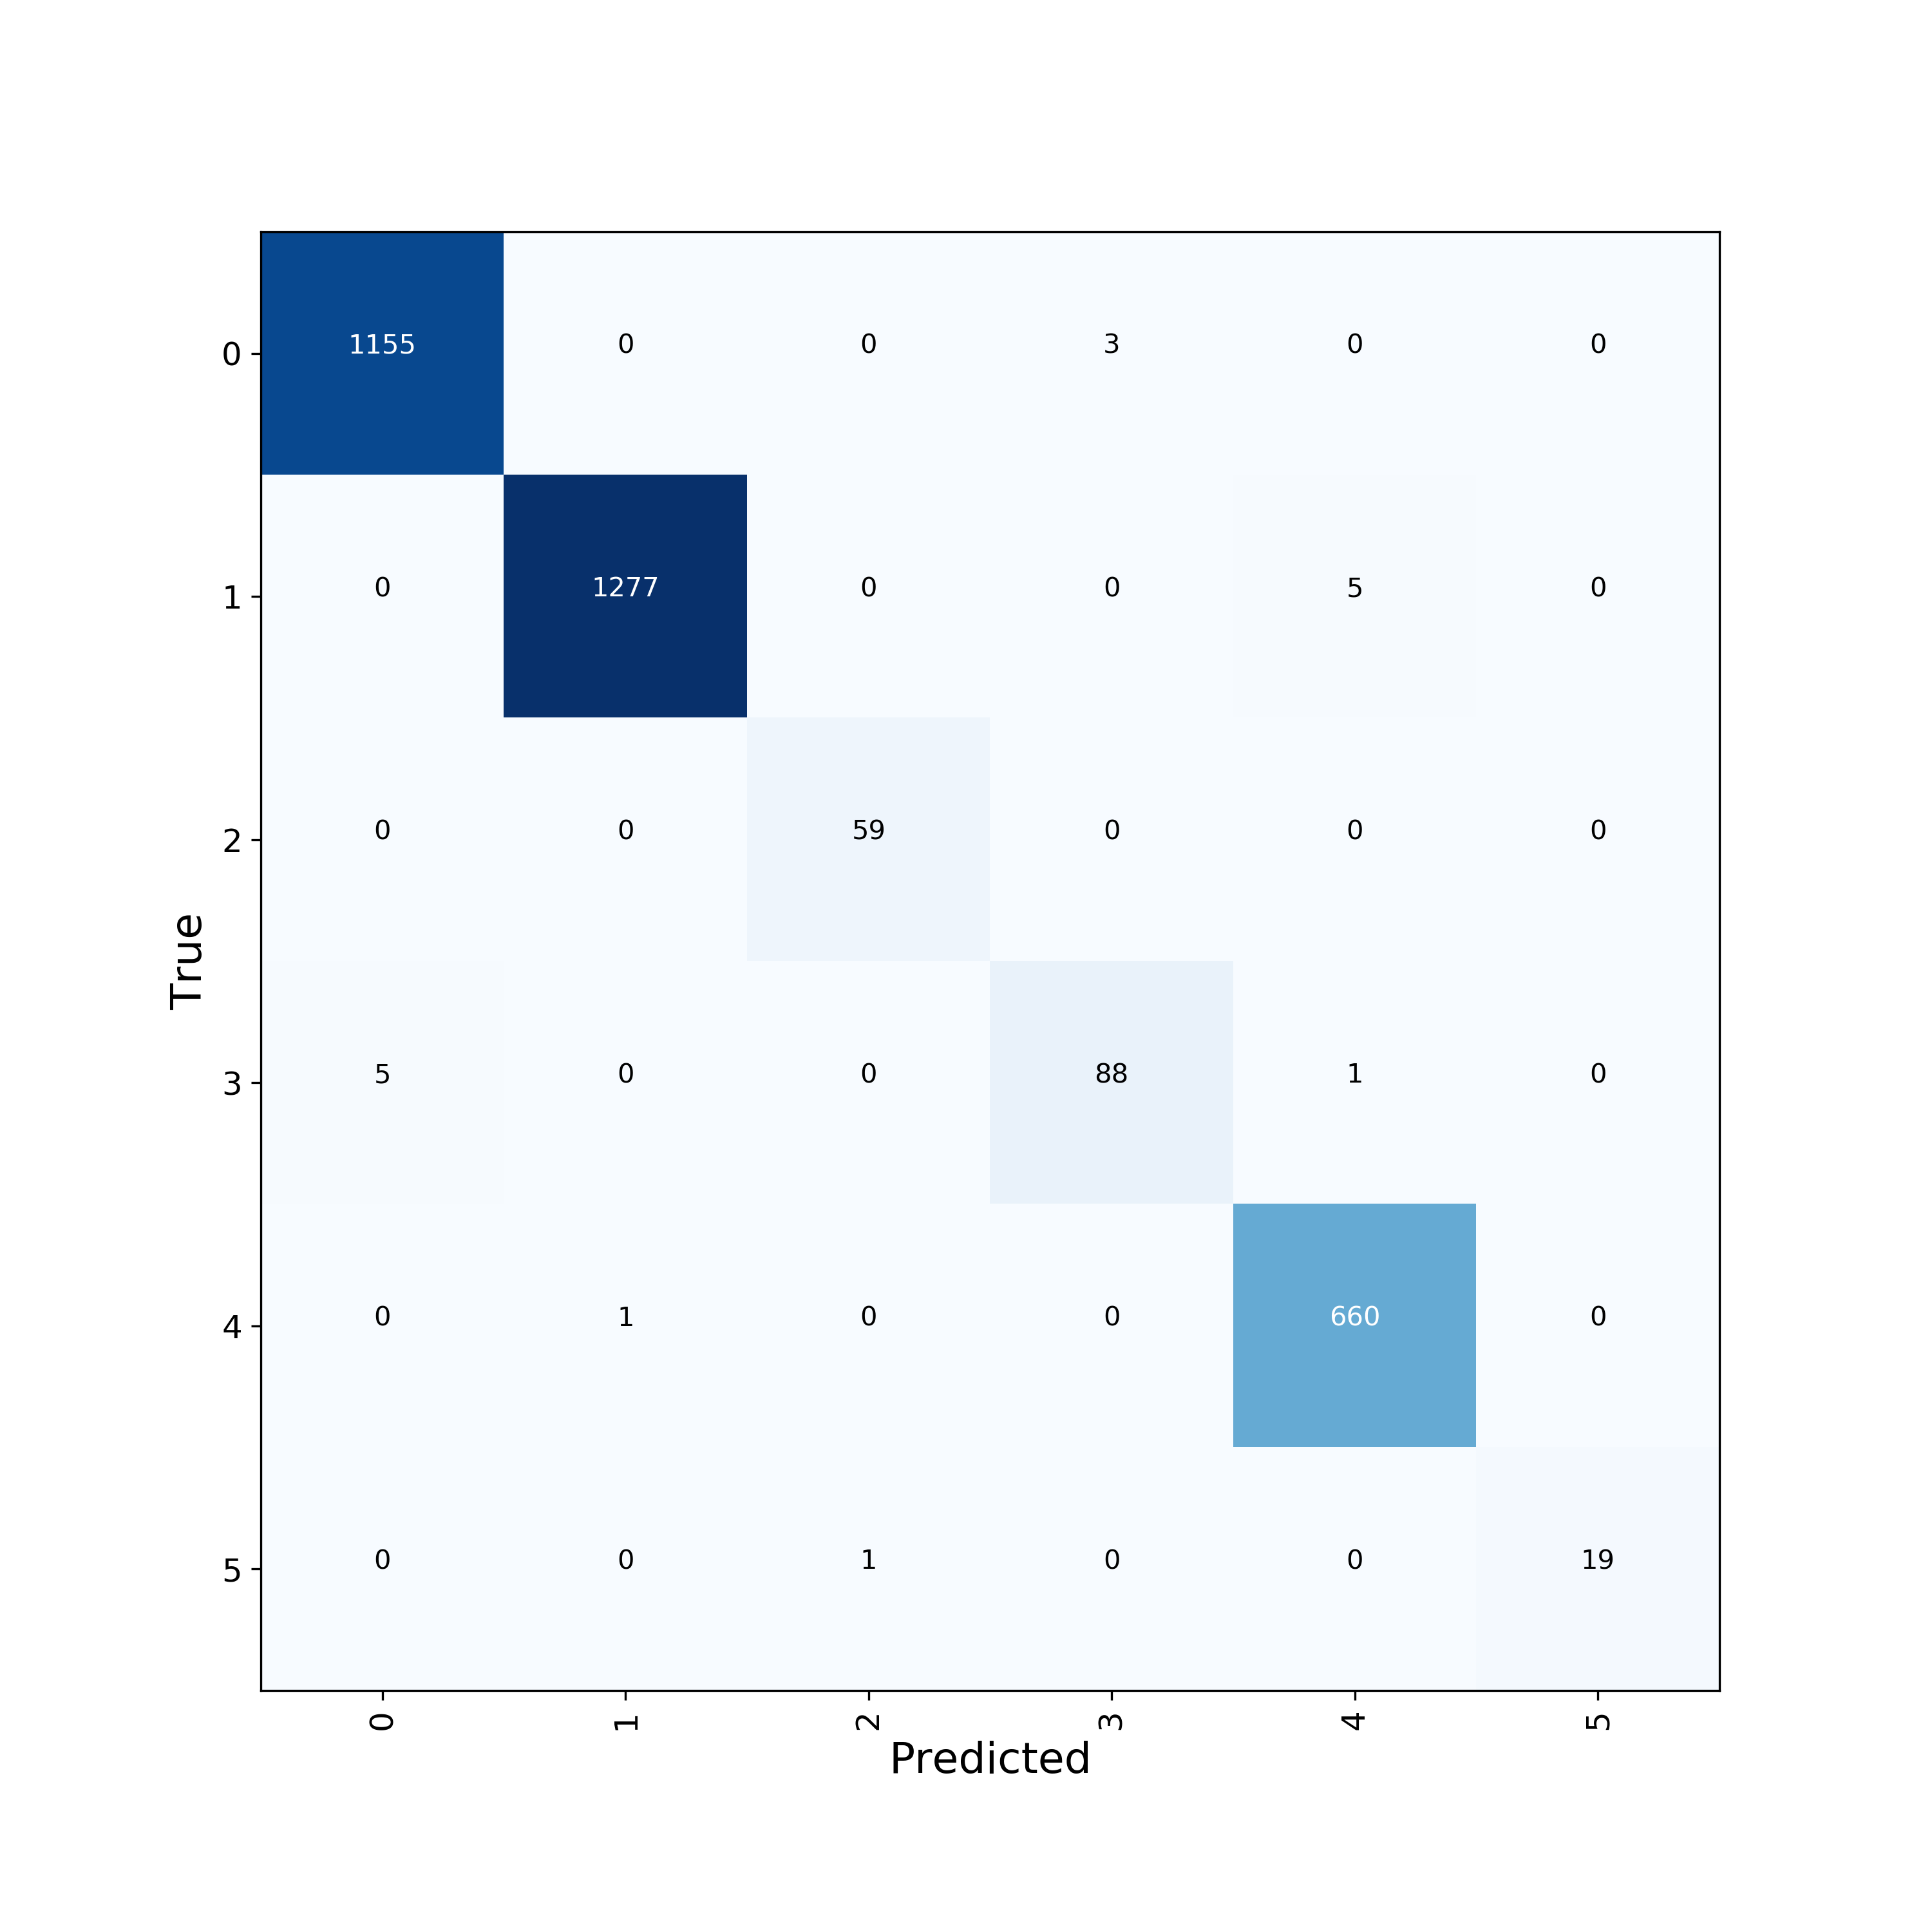
\includegraphics[width=1.0\linewidth]{confusion_matrix_traffic_light.png}
    \centering
    \caption{Testing confusion matrix with LISA traffic light}
    \label{fig:fig_13}
  \end{minipage}
\end{figure}

\section*{References}

% References follow the acknowledgments. Use unnumbered first-level
% heading for the references. Any choice of citation style is acceptable
% as long as you are consistent. It is permissible to reduce the font
% size to \verb+small+ (9 point) when listing the references. {\bf
%   Remember that you can use more than eight pages as long as the
%   additional pages contain \emph{only} cited references.}
\medskip

\small

[1] Angelova,A., Krizhevsky, A., Vanhoucke, V. Real-Time Pedestrian Detection With Deep Network Cascades. {\it Google research.}

[2] Habibi Aghdam,H., Jahani Heravi,E., Puig,D. (2016) A practical Approach for Detection and Classification of Traffic signs using Convolutional Neural Networks. {\it Robotics and Autonomous System}, Vol. 84, pp. 97-112.

[3] Kardkovacs, Z.T., Paroczi, Z.,Siegler,A.,(2011) Real-Time Traffic Sign Recognition System. {\it 2nd International Conference on Cognitive Infocommunications.}

[4] Shustanov, A., Yakimov, P., (2017). CNN Design For Real-Time Traffic Sign Recognition. {\it Procedia Engineering.} Vol.201,pp.718-725.

[5] Simonyan, K., Zisserman, A., (2014). Very Deep Convolutional Networks for Large-Scale Image Recognition. {\it ARXIV.} eprint arXiv:1409.1556

%% Zhu, Y.Y., Zhang, C.Q., Zhou, D.Y., Wang, X.G., Bai, X., Liu, W.Y., (2016) Traffic Sign Detection and Recognition Using Fully Convolutional Network Guided Proposals. {\it Neurocomputing.} Vol.214,pp.758-766.

%% Hasselmo, M.E., Schnell, E.\ \& Barkai, E.\ (1995) Dynamics of
%% learning and recall at excitatory recurrent synapses and cholinergic
%% modulation in rat hippocampal region CA3. {\it Journal of
%% Neuroscience} {\bf 15}(7):5249-5262.

\end{document}